\documentclass[11pt, letterpaper]{article}

% Fonts and Encoding
\usepackage[utf8]{inputenc}
\usepackage[T1]{fontenc}
\usepackage{lmodern} % High-quality Latin Modern vector font

% Math and Symbols
\usepackage{amsmath, amssymb, amsthm, amsfonts, mathrsfs, mathtools}

% Layout and Geometry
\usepackage{geometry}
\geometry{letterpaper, margin=1in}
\setlength{\parindent}{0pt}
\setlength{\parskip}{0.6em}

% Formatting and Graphics
\usepackage{graphicx, xcolor, enumitem, booktabs, array, tabularx}

% TikZ for Illustrations
\usepackage{tikz}
\usetikzlibrary{arrows.meta, positioning, shapes.geometric, calc, backgrounds, matrix}

% Clickable Links and TOC
\usepackage{hyperref}
\hypersetup{
    colorlinks=true,
    linkcolor=blue,
    filecolor=magenta,      
    urlcolor=cyan,
    pdftitle={Uncountable Sets},
}

% Theorem Environments
\newtheorem{theorem}{Theorem}[section]
\newtheorem{lemma}[theorem]{Lemma}
\newtheorem{proposition}[theorem]{Proposition}
\newtheorem{corollary}[theorem]{Corollary}
\theoremstyle{definition}
\newtheorem{definition}{Definition}[section]
\newtheorem{axiom}{Axiom}[section]
\newtheorem{example}{Example}[section]
\theoremstyle{remark}
\newtheorem{remark}{Remark}[section]

% Custom Commands (Enforced standard notation)
\newcommand{\R}{\mathbb{R}}
\newcommand{\N}{\mathbb{N}}
\newcommand{\Z}{\mathbb{Z}}
\newcommand{\Q}{\mathbb{Q}}
\newcommand{\E}{\mathbb{E}}
\newcommand{\Prob}{\mathbb{P}}
\newcommand{\F}{\mathcal{F}}

\title{\textbf{Advanced Masterclass on Uncountable Sets}\\
\large Section 11.3: Foundations of Transfinite Cardinality, Continuum Bijections, and Quantitative Modeling}
\author{Tashfeen Omran}
\date{\today}

\begin{document}

\maketitle
\tableofcontents
\newpage

\section{Comprehensive Introduction, Context, and Prerequisites}

\subsection{Core Concepts and Axioms}

In elementary set theory, the size of a finite set is captured unambiguously by a non-negative integer. When transitioning to infinite sets, naive counting breaks down, and mathematicians replace counting with \emph{bijective correspondence}. The theory of \textbf{Uncountable Sets} marks one of the most profound conceptual leaps in modern mathematics: the rigorous discovery that \emph{infinity is not monolithic}, and that strictly distinct hierarchies of infinite cardinality exist.

We formalize the foundational definitions governing Section 11.3 below, adopting the standard convention $\mathbb{N} = \{1, 2, 3, \dots\}$ for the set of natural numbers (positive integers).

\begin{definition}[Numerical Equivalence and Same Cardinality]
Two nonempty sets $A$ and $B$ are said to be \emph{numerically equivalent} (or to have the \emph{same cardinality}), written $|A| = |B|$, if and only if there exists a bijective function (both injective and surjective) $f : A \to B$. By convention, $|\emptyset| = |\emptyset|$.
\end{definition}

\begin{definition}[Denumerable, Countable, and Uncountable Sets]
Let $S$ be a set.
\begin{enumerate}[label=(\roman*)]
    \item $S$ is \emph{denumerable} (or \emph{countably infinite}) if $|S| = |\mathbb{N}|$; that is, there exists a bijection $f : \mathbb{N} \to S$.
    \item $S$ is \emph{countable} if $S$ is either finite or denumerable.
    \item $S$ is \emph{uncountable} if $S$ is not countable. Equivalently, $S$ is an infinite set for which no bijection $f : \mathbb{N} \to S$ exists.
\end{enumerate}
\end{definition}

\begin{definition}[Open Intervals of Real Numbers]
For any two real numbers $a, b \in \mathbb{R}$ with $a < b$, the \emph{open interval} $(a, b)$ is defined by
\[
(a, b) = \{x \in \mathbb{R} : a < x < b\}.
\]
Similarly, the set of strictly positive real numbers is denoted $\mathbb{R}^+ = (0, \infty) = \{x \in \mathbb{R} : x > 0\}$.
\end{definition}

A critical analytic prerequisite for proving the uncountability of the continuum $(0, 1)$ is the canonical representation of real numbers via base-$10$ decimal expansions.

\begin{axiom}[Decimal Expansion Structure of Real Numbers]
Every real number $x \in (0, 1)$ admits a decimal expansion
\[
x = 0.d_1 d_2 d_3 \cdots = \sum_{k=1}^{\infty} \frac{d_k}{10^k}, \quad \text{where } d_k \in \{0, 1, 2, \dots, 9\} \text{ for all } k \in \mathbb{N}.
\]
Furthermore:
\begin{enumerate}[label=(\roman*)]
    \item Every irrational number $x \in (0, 1) \setminus \mathbb{Q}$ has a \emph{unique} decimal expansion, and this expansion is non-repeating (not eventually periodic).
    \item Every rational number $x \in (0, 1) \cap \mathbb{Q}$ has an eventually periodic decimal expansion. A reduced fraction $p/q \in (0, 1)$ (with $p, q \in \mathbb{N}$ and $\gcd(p, q) = 1$) possesses \emph{two} distinct decimal expansions if and only if the only prime factors of $q$ are $2$ and/or $5$; in this case, one expansion terminates (repeats the digit $0$ from some index onward), while the alternate expansion repeats the digit $9$ from some index onward (for example, $\frac{1}{2} = 0.5000\cdots = 0.4999\cdots$).
    \item If we restrict every real number in $(0, 1)$ to disallow expansions ending in an infinite string of $9$s, then the decimal expansion of every $x \in (0, 1)$ is \emph{strictly unique}.
\end{enumerate}
\end{axiom}

\subsection{Intuition and Set-Theoretic/Logical Foundations}

At first glance, the existence of uncountable sets defies physical and arithmetic intuition. Earlier investigations of denumerable sets reveal surprising absorptions of infinity: the integers $\mathbb{Z}$ and even the dense rational numbers $\mathbb{Q}$ can be placed in exact one-to-one correspondence with the natural numbers $\mathbb{N}$. One might naturally conjecture that \emph{every} infinite set can be sequentially listed as $\{a_1, a_2, a_3, \dots\}$.

Georg Cantor shattered this intuition via the \textbf{Diagonalization Principle}. Imagine attempting to catalog every point in the open unit interval $(0, 1)$ in an infinite ledger, row by row:
\begin{align*}
f(1) = a_1 &= 0.a_{11}a_{12}a_{13}\cdots \\
f(2) = a_2 &= 0.a_{21}a_{22}a_{23}\cdots \\
f(3) = a_3 &= 0.a_{31}a_{32}a_{33}\cdots \\
&\;\;\vdots
\end{align*}
Diagonalization exploits self-reference across the $n$-th digit of the $n$-th listed number. By constructing a new real number $b = 0.b_1 b_2 b_3 \cdots$ whose $i$-th digit $b_i$ deliberately disagrees with $a_{ii}$ (while carefully avoiding the digits $0$ and $9$ so that $b$ can never be an alternate decimal representation of any terminating rational), we engineer an adversarial counterexample that simultaneously evades \emph{every} row of the ledger. No matter how cleverly one attempts to enumerate $(0, 1)$, the list is structurally incomplete.

Equally counterintuitive is the geometric malleability of uncountable continua. Although the open interval $(0, 1)$ has finite Euclidean length $1$ and is a proper subset of $\mathbb{R}$, there exists a smooth, continuous stretching bijection (a homeomorphism) mapping $(-1, 1)$ and $(0, 1)$ onto the entire unbounded real line $\mathbb{R}$. Set-theoretic cardinality discards metric notions like length, distance, and boundedness; it preserves only pure point-to-point correspondence. Consequently, for infinite sets $C$ and $D$, strict containment $C \subset D$ does \emph{not} preclude $|C| = |D|$ (as seen both in $\mathbb{Z} \subset \mathbb{Q}$ and in $(0, 1) \subset \mathbb{R}$), nor does an infinite subset of an uncountable set need to remain uncountable (for instance, $\mathbb{Z} \subset \mathbb{R}$ is infinite yet denumerable).

\subsection{Historical Context and Motivation}

The formal theory of uncountable sets originated with Georg Cantor in the late nineteenth century, emerging initially from an applied problem in mathematical analysis: determining the uniqueness sets for trigonometric (Fourier) series. In December 1873, Cantor proved that the algebraic numbers are countable, and in his landmark 1874 paper \emph{\"Uber eine Eigenschaft des Inbegriffes aller reellen algebraischen Zahlen}, he proved the uncountability of $\mathbb{R}$ using a nested closed-interval construction—immediately yielding a non-constructive proof of the existence of transcendental numbers without exhibiting a single one.

In 1891, Cantor published his far more celebrated and general \textbf{diagonal argument}, demonstrating not only the uncountability of the continuum but also the existence of an unbounded hierarchy of transfinite cardinals. These results ignited a fierce foundational crisis in mathematics. Prominent constructivists such as Leopold Kronecker rejected completed infinities outright, while paradoxes in naive set theory (such as Russell's Paradox) forced mathematicians like Ernst Zermelo and Abraham Fraenkel to axiomatize set theory (ZFC). David Hilbert famously defended Cantor's legacy, declaring, \emph{``No one shall expel us from the paradise that Cantor has created.''} Today, the distinction between countable and uncountable sets forms the architectural backbone of Lebesgue measure theory, modern probability spaces, functional analysis, and computability theory.

\subsection{Key Theorems, Lemmas, and Formulas}

The core results established in Section 11.3, along with the foundational lemmas from earlier sections upon which their proofs depend, are compiled below.

\begin{theorem}[Infinite Subsets of Denumerable Sets — Prerequisite Theorem 11.4]
Every infinite subset of a denumerable set is denumerable. Equivalently, every subset of a countable set is countable.
\end{theorem}

\begin{theorem}[Closure of Bijections Under Inversion and Composition — Prerequisite Results]
If $f : A \to B$ is bijective, then its inverse $f^{-1} : B \to A$ is bijective. Moreover, if $f : A \to B$ and $g : B \to C$ are bijective, then their composition $g \circ f : A \to C$ is bijective.
\end{theorem}

\begin{theorem}[Cantor's Uncountability Theorem — Theorem 11.9]
The open interval $(0, 1)$ of real numbers is uncountable.
\end{theorem}

\begin{theorem}[Upward Monotonicity of Uncountability — Theorem 11.10]
Let $A$ and $B$ be sets such that $A \subseteq B$. If $A$ is uncountable, then $B$ is uncountable.
\end{theorem}

\begin{corollary}[Uncountability of the Real Line — Corollary 11.11]
The set $\mathbb{R}$ of real numbers is uncountable.
\end{corollary}

\begin{theorem}[Equivalence of Denumerable Sets — Theorem 11.12]
Every two denumerable sets are numerically equivalent. That is, if $A$ and $B$ are denumerable, then $|A| = |B|$.
\end{theorem}

\begin{theorem}[Separation of Denumerable and Uncountable Cardinalities — Theorem 11.13]
If $A$ is a denumerable set and $B$ is an uncountable set, then $A$ and $B$ are not numerically equivalent; that is, $|A| \neq |B|$.
\end{theorem}

\begin{theorem}[Numerical Equivalence of $(-1, 1)$ and $\mathbb{R}$ — Theorem 11.14]
The sets $(-1, 1)$ and $\mathbb{R}$ are numerically equivalent. In particular, the explicit function $f : (-1, 1) \to \mathbb{R}$ defined by
\[
f(x) = \frac{x}{1 - |x|}
\]
is a bijection.
\end{theorem}

\begin{corollary}[Numerical Equivalence of $(0, 1)$ and $\mathbb{R}$ — Corollary 11.15]
The sets $(0, 1)$ and $\mathbb{R}$ are numerically equivalent.
\end{corollary}

\subsection{Prerequisites}

To master Section 11.3 and execute its proofs without logical gaps, the reader must be fluent in the following foundational skills:
\begin{itemize}
    \item \textbf{Proof Techniques:} Direct proof, proof by contradiction (\emph{reductio ad absurdum}), case analysis (sign splits for absolute values and inequalities), and constructive existence proofs.
    \item \textbf{Function Theory:} Rigorous verification of well-definedness, injectivity ($f(a) = f(b) \implies a = b$), surjectivity ($\forall y \in B,\ \exists x \in A \text{ such that } f(x) = y$), function inverses, and compositions.
    \item \textbf{Countable Set Theory:} Familiarity with the countability of $\mathbb{N}$, $\mathbb{Z}$, and $\mathbb{Q}$, the closure of countable sets under finite/countable unions, and the equivalence relation properties of numerical equivalence ($|A| = |B|$).
    \item \textbf{Real Algebra and Order Properties:} Manipulating strict inequalities, absolute values, quadratic equations, and elementary transcendental functions ($\exp$, $\ln$).
\end{itemize}

\section{Detailed Homework Solutions}

In this section, we present complete, rigorous solutions to every exercise in Section 11.3 (Exercises 11.20 through 11.25). Each problem statement is reproduced verbatim prior to its proof.

\subsection{Exercise 11.20}

\textbf{Original Problem:} Prove that the set of irrational numbers is uncountable.

\medskip
\textbf{Proof Technique:} Proof by Contradiction, supported by an explicit lemma establishing that the union of two countable sets is countable.

\medskip
\begin{lemma}[Union of Two Disjoint Countable Sets]
Let $A$ and $B$ be disjoint sets ($A \cap B = \emptyset$). If $A$ is denumerable and $B$ is countable, then $A \cup B$ is denumerable (and hence countable).
\end{lemma}

\begin{proof}[Proof of Lemma]
Since $A$ is denumerable, there exists a bijection $f : \mathbb{N} \to A$, so we may list $A = \{a_1, a_2, a_3, \dots\}$ where $a_n = f(n)$ and $a_i \neq a_j$ for $i \neq j$. Since $B$ is countable, $B$ is either finite or denumerable. We examine both cases:

\textbf{Case 1:} $B$ is finite. If $B = \emptyset$, then $A \cup B = A$ is immediately denumerable. Otherwise, suppose $|B| = m$ for some $m \in \mathbb{N}$, so $B = \{b_1, b_2, \dots, b_m\}$ with distinct elements. Define $h : \mathbb{N} \to A \cup B$ by
\[
h(n) = \begin{cases}
b_n & \text{if } 1 \le n \le m, \\
a_{n-m} & \text{if } n > m.
\end{cases}
\]
Because $A \cap B = \emptyset$, the images of $\{1, \dots, m\}$ and $\{m+1, m+2, \dots\}$ are disjoint; since $n \mapsto b_n$ is injective on $\{1, \dots, m\}$ and $n \mapsto a_{n-m}$ is injective on $\{m+1, m+2, \dots\}$, $h$ is injective. Moreover, every $b_k \in B$ equals $h(k)$ and every $a_j \in A$ equals $h(j+m)$, so $h$ is surjective. Thus $h$ is bijective and $A \cup B$ is denumerable.

\textbf{Case 2:} $B$ is denumerable. Then there exists a bijection $g : \mathbb{N} \to B$, so $B = \{b_1, b_2, b_3, \dots\}$ with $b_i \neq b_j$ for $i \neq j$. Define $h : \mathbb{N} \to A \cup B$ by interleaving odd and even indices:
\[
h(n) = \begin{cases}
a_{(n+1)/2} & \text{if } n \text{ is odd}, \\
b_{n/2} & \text{if } n \text{ is even}.
\end{cases}
\]
To verify injectivity, suppose $h(n_1) = h(n_2)$ for $n_1, n_2 \in \mathbb{N}$. Since $A \cap B = \emptyset$, $n_1$ and $n_2$ must have the same parity. If both are odd, then $a_{(n_1+1)/2} = a_{(n_2+1)/2}$, so $(n_1+1)/2 = (n_2+1)/2$ by injectivity of $f$, giving $n_1 = n_2$. If both are even, then $b_{n_1/2} = b_{n_2/2}$, so $n_1/2 = n_2/2$ by injectivity of $g$, giving $n_1 = n_2$. To verify surjectivity, let $x \in A \cup B$. If $x \in A$, then $x = a_k$ for some $k \in \mathbb{N}$, so $h(2k - 1) = a_k = x$. If $x \in B$, then $x = b_k$ for some $k \in \mathbb{N}$, so $h(2k) = b_k = x$. Thus $h$ is bijective, and $A \cup B$ is denumerable.
\end{proof}

\begin{proof}[Proof of Exercise 11.20]
Let $\mathbb{I} = \mathbb{R} \setminus \mathbb{Q}$ denote the set of irrational numbers. Assume, to the contrary, that $\mathbb{I}$ is countable.

Recall from the definition of irrational numbers that $\mathbb{Q}$ and $\mathbb{I}$ partition the real line:
\[
\mathbb{R} = \mathbb{Q} \cup \mathbb{I} \quad \text{and} \quad \mathbb{Q} \cap \mathbb{I} = \emptyset.
\]
We know from prior results on countable sets that the set of rational numbers $\mathbb{Q}$ is denumerable. Under our assumption that $\mathbb{I}$ is countable, applying the Lemma above to the disjoint sets $A = \mathbb{Q}$ (denumerable) and $B = \mathbb{I}$ (countable) implies that $\mathbb{R} = \mathbb{Q} \cup \mathbb{I}$ is denumerable, and therefore countable.

However, by Corollary 11.11, the set $\mathbb{R}$ of real numbers is uncountable. This yields a contradiction. Hence, our assumption is false, and the set of irrational numbers $\mathbb{I}$ is uncountable.
\end{proof}

\subsection{Exercise 11.21}

\textbf{Original Problem:} Prove that the set of complex numbers is uncountable.

\medskip
\textbf{Proof Technique:} Direct Proof using Upward Monotonicity of Uncountability (Theorem 11.10) and Corollary 11.11.

\begin{proof}[Proof of Exercise 11.21]
Recall that the set of complex numbers is defined by
\[
\mathbb{C} = \{a + bi : a, b \in \mathbb{R}\}, \quad \text{where } i^2 = -1.
\]
Every real number $a \in \mathbb{R}$ is identified with the complex number $a + 0i \in \mathbb{C}$, which establishes the subset inclusion
\[
\mathbb{R} \subseteq \mathbb{C}.
\]
(Note: If one adopts the formal Cartesian construction $\mathbb{C} = \mathbb{R} \times \mathbb{R}$, then the map $\iota : \mathbb{R} \to \mathbb{R} \times \{0\}$ defined by $\iota(a) = (a, 0)$ is bijective; since $\mathbb{R}$ is uncountable by Corollary 11.11, $\mathbb{R} \times \{0\}$ is uncountable by Theorem 11.13, and $\mathbb{R} \times \{0\} \subseteq \mathbb{C}$.)

By Corollary 11.11, the set $\mathbb{R}$ is uncountable. Since $\mathbb{R} \subseteq \mathbb{C}$ and $\mathbb{R}$ is uncountable, it follows directly from Theorem 11.10 that the set $\mathbb{C}$ of complex numbers is uncountable.
\end{proof}

\subsection{Exercise 11.22}

\textbf{Original Problem:} Prove that the open interval $(-2, 2)$ and $\mathbb{R}$ are numerically equivalent by finding a bijective function $h : (-2, 2) \to \mathbb{R}$. (Show that your function is, in fact, bijective.)

\medskip
\textbf{Proof Technique:} Constructive Direct Proof (exhibiting an explicit algebraic bijection and proving well-definedness, injectivity, and surjectivity directly).

\begin{proof}[Proof of Exercise 11.22]
Define the function $h : (-2, 2) \to \mathbb{R}$ by
\[
h(x) = \frac{x}{2 - |x|}.
\]
(Intuitively, this function arises by scaling $(-2, 2)$ onto $(-1, 1)$ via $u = x/2$ and applying the canonical bijection $f(u) = \frac{u}{1 - |u|}$ from Theorem 11.14.)

\textbf{Step 1: Well-Definedness.} Let $x \in (-2, 2)$. Then $-2 < x < 2$, which is equivalent to $|x| < 2$. Consequently, $2 - |x| > 0$, so the denominator never vanishes. Thus $h(x)$ is a uniquely determined real number for every $x \in (-2, 2)$.

\textbf{Step 2: Injectivity (One-to-One).} Let $a, b \in (-2, 2)$ and suppose that $h(a) = h(b)$. Then
\[
\frac{a}{2 - |a|} = \frac{b}{2 - |b|}.
\]
Because $2 - |a| > 0$ and $2 - |b| > 0$, the sign of $h(x)$ matches the sign of $x$ for every $x \in (-2, 2)$. We therefore partition into three mutually exclusive and exhaustive cases based on the common value $v = \frac{a}{2 - |a|} = \frac{b}{2 - |b|}$:
\begin{itemize}
    \item \emph{Case 1 ($v = 0$):} Since the denominators are strictly positive, $\frac{a}{2 - |a|} = 0$ and $\frac{b}{2 - |b|} = 0$ immediately yield $a = 0$ and $b = 0$, hence $a = b$.
    \item \emph{Case 2 ($v > 0$):} Since the denominators are strictly positive, we must have $a > 0$ and $b > 0$. Therefore $|a| = a$ and $|b| = b$, so
    \[
    \frac{a}{2 - a} = \frac{b}{2 - b}.
    \]
    Cross-multiplying gives $a(2 - b) = b(2 - a)$, which expands to $2a - ab = 2b - ab$. Adding $ab$ to both sides yields $2a = 2b$, and dividing by $2$ gives $a = b$.
    \item \emph{Case 3 ($v < 0$):} Since the denominators are strictly positive, we must have $a < 0$ and $b < 0$. Therefore $|a| = -a$ and $|b| = -b$, so
    \[
    \frac{a}{2 + a} = \frac{b}{2 + b}.
    \]
    Cross-multiplying gives $a(2 + b) = b(2 + a)$, which expands to $2a + ab = 2b + ab$. Subtracting $ab$ from both sides yields $2a = 2b$, and dividing by $2$ gives $a = b$.
\end{itemize}
In all three cases, $a = b$. Thus $h$ is injective.

\textbf{Step 3: Surjectivity (Onto).} Let $r \in \mathbb{R}$ be arbitrary. We must exhibit $x \in (-2, 2)$ such that $h(x) = r$. We consider three exhaustive cases:
\begin{itemize}
    \item \emph{Case 1 ($r = 0$):} Choose $x = 0 \in (-2, 2)$. Then
    \[
    h(0) = \frac{0}{2 - |0|} = \frac{0}{2} = 0 = r.
    \]
    \item \emph{Case 2 ($r > 0$):} Choose $x = \frac{2r}{1 + r}$. Since $r > 0$, we have $1 + r > 1 > 0$ and $0 < r < 1 + r$. Multiplying by $2$ and dividing by $1 + r > 0$ gives
    \[
    0 < \frac{2r}{1 + r} < 2,
    \]
    so $x \in (0, 2) \subset (-2, 2)$. Because $x > 0$, $|x| = x$, and therefore
    \[
    h(x) = \frac{\frac{2r}{1 + r}}{2 - \frac{2r}{1 + r}} = \frac{\frac{2r}{1 + r}}{\frac{2(1 + r) - 2r}{1 + r}} = \frac{2r}{2 + 2r - 2r} = \frac{2r}{2} = r.
    \]
    \item \emph{Case 3 ($r < 0$):} Choose $x = \frac{2r}{1 - r}$. Since $r < 0$, we have $-r > 0$, hence $1 - r > 1 > 0$. Moreover, $2r < 0$, and adding $-2 < 0$ to $2r$ shows $-2 + 2r < 2r$, i.e., $-2(1 - r) < 2r < 0$. Dividing by $1 - r > 0$ yields
    \[
    -2 < \frac{2r}{1 - r} < 0,
    \]
    so $x \in (-2, 0) \subset (-2, 2)$. Because $x < 0$, $|x| = -x = \frac{-2r}{1 - r}$, and therefore
    \[
    h(x) = \frac{\frac{2r}{1 - r}}{2 - \left(\frac{-2r}{1 - r}\right)} = \frac{\frac{2r}{1 - r}}{\frac{2(1 - r) + 2r}{1 - r}} = \frac{2r}{2 - 2r + 2r} = \frac{2r}{2} = r.
    \]
\end{itemize}
Thus, for every $r \in \mathbb{R}$, there exists $x \in (-2, 2)$ with $h(x) = r$, proving that $h$ is surjective.

\textbf{Conclusion:} Since $h : (-2, 2) \to \mathbb{R}$ is both injective and surjective, it is bijective. By the definition of numerical equivalence, $(-2, 2)$ and $\mathbb{R}$ are numerically equivalent ($|(-2, 2)| = |\mathbb{R}|$).
\end{proof}

\subsection{Exercise 11.23}

\textbf{Original Problem:}
\begin{enumerate}[label=(\alph*)]
    \item Prove that the function $f : (0, 1) \to (0, 2)$, mapping the open interval $(0, 1)$ into the open interval $(0, 2)$ and defined by $f(x) = 2x$, is bijective.
    \item Explain why $(0, 1)$ and $(0, 2)$ have the same cardinality.
    \item Let $a, b \in \mathbb{R}$, where $a < b$. Prove that $(0, 1)$ and $(a, b)$ have the same cardinality.
\end{enumerate}

\medskip
\textbf{Proof Technique:} Direct Proof via explicit verification of linear and affine bijections.

\begin{proof}[Solution to Exercise 11.23]
\textbf{Part (a):} Consider $f : (0, 1) \to (0, 2)$ given by $f(x) = 2x$.
\begin{itemize}
    \item \emph{Well-Definedness:} Let $x \in (0, 1)$, so $0 < x < 1$. Multiplying all terms of this strict inequality by the positive constant $2$ gives $0 < 2x < 2$, which implies $f(x) \in (0, 2)$.
    \item \emph{Injectivity:} Let $x_1, x_2 \in (0, 1)$ such that $f(x_1) = f(x_2)$. Then $2x_1 = 2x_2$. Dividing both sides by $2 \neq 0$ yields $x_1 = x_2$. Hence $f$ is one-to-one.
    \item \emph{Surjectivity:} Let $y \in (0, 2)$ be arbitrary, so $0 < y < 2$. Define $x = \frac{y}{2}$. Dividing the strict inequality $0 < y < 2$ by $2 > 0$ gives $0 < \frac{y}{2} < 1$, so $x \in (0, 1)$. Furthermore,
    \[
    f(x) = 2\left(\frac{y}{2}\right) = y.
    \]
    Hence $f$ is onto.
\end{itemize}
Since $f$ is both one-to-one and onto, $f : (0, 1) \to (0, 2)$ is bijective.

\medskip
\textbf{Part (b):} By definition, two nonempty sets $A$ and $B$ have the same cardinality (are numerically equivalent, $|A| = |B|$) if and only if there exists a bijective function mapping $A$ onto $B$. Because $(0, 1)$ and $(0, 2)$ are nonempty and Part (a) explicitly established that $f : (0, 1) \to (0, 2)$ defined by $f(x) = 2x$ is bijective, it follows directly from the definition that $(0, 1)$ and $(0, 2)$ have the same cardinality: $|(0, 1)| = |(0, 2)|$.

\medskip
\textbf{Part (c):} Let $a, b \in \mathbb{R}$ with $a < b$. Then $b - a > 0$. Define the affine linear map $\varphi : (0, 1) \to (a, b)$ by
\[
\varphi(x) = (b - a)x + a.
\]
\begin{itemize}
    \item \emph{Well-Definedness:} Let $x \in (0, 1)$, so $0 < x < 1$. Since $b - a > 0$, multiplying through by $b - a$ preserves strict inequalities:
    \[
    0 < (b - a)x < b - a.
    \]
    Adding $a$ to all parts yields
    \[
    a < (b - a)x + a < b,
    \]
    which confirms that $\varphi(x) \in (a, b)$ for all $x \in (0, 1)$.
    \item \emph{Injectivity:} Let $x_1, x_2 \in (0, 1)$ such that $\varphi(x_1) = \varphi(x_2)$. Then
    \[
    (b - a)x_1 + a = (b - a)x_2 + a.
    \]
    Subtracting $a$ from both sides gives $(b - a)x_1 = (b - a)x_2$. Because $a < b$, we have $b - a \neq 0$, so dividing both sides by $b - a$ yields $x_1 = x_2$. Therefore, $\varphi$ is injective.
    \item \emph{Surjectivity:} Let $y \in (a, b)$ be arbitrary, so $a < y < b$. Define
    \[
    x = \frac{y - a}{b - a}.
    \]
    Subtracting $a$ from $a < y < b$ yields $0 < y - a < b - a$. Dividing by $b - a > 0$ gives
    \[
    0 < \frac{y - a}{b - a} < 1,
    \]
    so $x \in (0, 1)$. Evaluating $\varphi$ at $x$ gives
    \[
    \varphi(x) = (b - a)\left(\frac{y - a}{b - a}\right) + a = (y - a) + a = y.
    \]
    Therefore, $\varphi$ is surjective.
\end{itemize}
Since $\varphi : (0, 1) \to (a, b)$ is bijective, the open intervals $(0, 1)$ and $(a, b)$ have the same cardinality: $|(0, 1)| = |(a, b)|$.
\end{proof}

\subsection{Exercise 11.24}

\textbf{Original Problem:} Prove that $\mathbb{R}$ and $\mathbb{R}^+$ are numerically equivalent.

\medskip
\textbf{Proof Technique:} Constructive Direct Proof via the natural exponential bijection $f : \mathbb{R} \to \mathbb{R}^+$.

\begin{proof}[Proof of Exercise 11.24]
Recall that $\mathbb{R}^+ = (0, \infty) = \{y \in \mathbb{R} : y > 0\}$. Define the function $f : \mathbb{R} \to \mathbb{R}^+$ by
\[
f(x) = e^x.
\]
\begin{itemize}
    \item \emph{Well-Definedness:} For every real number $x \in \mathbb{R}$, $e^x$ is a strictly positive real number ($e^x > 0$). Hence $f(x) \in \mathbb{R}^+$ for all $x \in \mathbb{R}$.
    \item \emph{Injectivity:} Let $x_1, x_2 \in \mathbb{R}$ and suppose $f(x_1) = f(x_2)$, so that $e^{x_1} = e^{x_2}$. Since both sides lie in $\mathbb{R}^+$, we may apply the natural logarithm function $\ln : \mathbb{R}^+ \to \mathbb{R}$ to both sides:
    \[
    \ln\left(e^{x_1}\right) = \ln\left(e^{x_2}\right) \implies x_1 = x_2.
    \]
    (Equivalently, $f'(x) = e^x > 0$ for all $x \in \mathbb{R}$, so $f$ is strictly increasing and therefore injective.)
    \item \emph{Surjectivity:} Let $y \in \mathbb{R}^+$ be arbitrary. Because $y > 0$, the natural logarithm $x = \ln(y)$ is a well-defined real number ($x \in \mathbb{R}$). Moreover,
    \[
    f(x) = e^{\ln(y)} = y.
    \]
    Hence $f$ is surjective.
\end{itemize}
Because $f : \mathbb{R} \to \mathbb{R}^+$ is both injective and surjective, it is bijective. Therefore, $\mathbb{R}$ and $\mathbb{R}^+$ are numerically equivalent ($|\mathbb{R}| = |\mathbb{R}^+|$).
\end{proof}

\begin{remark}
One can also prove $|\mathbb{R}| = |\mathbb{R}^+|$ purely algebraically without transcendental functions: first verify that $\psi : (0, 1) \to \mathbb{R}^+$ given by $\psi(t) = \frac{t}{1 - t}$ is a bijection (with inverse $\psi^{-1}(y) = \frac{y}{1 + y}$), and then compose $\psi$ with the bijection $\mathbb{R} \to (0, 1)$ obtained from Corollary 11.15.
\end{remark}

\subsection{Exercise 11.25}

\textbf{Original Problem:} Consider the function $g : (-1, 1) \to \mathbb{R}$ defined by $g(x) = \frac{x}{1 - x^2}$.
\begin{enumerate}[label=(\alph*)]
    \item Prove that $g$ is onto.
    \item Prove that $g$ is one-to-one.
    \item From the information obtained in (a) and (b), what conclusion can be made?
\end{enumerate}

\medskip
\textbf{Proof Technique:} Purely Algebraic Direct Proof (solving a quadratic equation with strict domain verification for surjectivity, and using algebraic factorization with an absolute-value bound for injectivity).

\begin{proof}[Solution to Exercise 11.25]
First observe that $g$ is well-defined on $(-1, 1)$: for any $x \in (-1, 1)$, $|x| < 1 \implies 0 \le x^2 < 1 \implies 1 - x^2 > 0$, so the denominator is strictly positive and $g(x) \in \mathbb{R}$.

\medskip
\textbf{Part (a): Proof that $g$ is onto (surjective).} Let $r \in \mathbb{R}$ be arbitrary. We must find $x \in (-1, 1)$ such that $\frac{x}{1 - x^2} = r$. We treat $r = 0$ and $r \neq 0$ separately.

\emph{Case 1 ($r = 0$):} Choose $x = 0 \in (-1, 1)$. Then
\[
g(0) = \frac{0}{1 - 0^2} = 0 = r.
\]

\emph{Case 2 ($r \neq 0$):} Notice that solving $\frac{x}{1 - x^2} = r$ rearranges to the quadratic equation $rx^2 + x - r = 0$, whose discriminant is $\Delta = 1^2 - 4(r)(-r) = 1 + 4r^2 > 1$. Guided by the quadratic formula, define
\[
x = \frac{-1 + \sqrt{1 + 4r^2}}{2r}.
\]
We must verify \emph{two} essential properties: (i) $x \in (-1, 1)$, and (ii) $g(x) = r$.

\emph{Verification of (i):} Since $r \neq 0$, we have $|r| > 0$ and $4r^2 > 0$. Therefore, $1 + 4r^2 > 1$, so taking positive square roots gives $\sqrt{1 + 4r^2} > 1$, meaning $-1 + \sqrt{1 + 4r^2} > 0$. Next, compare $1 + 4r^2$ with $(1 + 2|r|)^2$:
\[
(1 + 2|r|)^2 = 1 + 4|r| + 4r^2 > 1 + 4r^2 \quad (\text{since } 4|r| > 0).
\]
Since both sides are strictly positive, taking square roots preserves the strict inequality:
\[
\sqrt{1 + 4r^2} < 1 + 2|r| \implies 0 < -1 + \sqrt{1 + 4r^2} < 2|r|.
\]
Dividing through by $2|r| > 0$, we obtain
\[
|x| = \left|\frac{-1 + \sqrt{1 + 4r^2}}{2r}\right| = \frac{-1 + \sqrt{1 + 4r^2}}{2|r|} < 1.
\]
Hence $-1 < x < 1$, confirming that $x \in (-1, 1)$.

\emph{Verification of (ii):} Compute $x^2$ and $1 - x^2$ explicitly:
\begin{align*}
x^2 &= \frac{\left(-1 + \sqrt{1 + 4r^2}\right)^2}{4r^2} = \frac{1 - 2\sqrt{1 + 4r^2} + (1 + 4r^2)}{4r^2} = \frac{2 + 4r^2 - 2\sqrt{1 + 4r^2}}{4r^2} \\
&= \frac{1 + 2r^2 - \sqrt{1 + 4r^2}}{2r^2}.
\end{align*}
Subtracting $x^2$ from $1$ yields
\[
1 - x^2 = \frac{2r^2 - \left(1 + 2r^2 - \sqrt{1 + 4r^2}\right)}{2r^2} = \frac{-1 + \sqrt{1 + 4r^2}}{2r^2}.
\]
Because $-1 + \sqrt{1 + 4r^2} > 0$ and $r \neq 0$, we compute $g(x)$ directly:
\[
g(x) = \frac{x}{1 - x^2} = \frac{\frac{-1 + \sqrt{1 + 4r^2}}{2r}}{\frac{-1 + \sqrt{1 + 4r^2}}{2r^2}} = \frac{2r^2}{2r} = r.
\]
In both cases, $r$ lies in the range of $g$. Thus, $g$ is onto.

\medskip
\textbf{Part (b): Proof that $g$ is one-to-one (injective).} Let $a, b \in (-1, 1)$ and suppose $g(a) = g(b)$. Then
\[
\frac{a}{1 - a^2} = \frac{b}{1 - b^2}.
\]
Since $1 - a^2 > 0$ and $1 - b^2 > 0$, cross-multiplying yields an equivalent equation:
\begin{align*}
a(1 - b^2) &= b(1 - a^2) \\
a - ab^2 &= b - a^2 b \\
(a - b) + ab(a - b) &= 0 \\
(a - b)(1 + ab) &= 0.
\end{align*}
Because $a, b \in (-1, 1)$, we have $|a| < 1$ and $|b| < 1$. Multiplying these non-negative inequalities gives
\[
|ab| = |a|\cdot|b| < 1 \cdot 1 = 1 \implies -1 < ab < 1 \implies 1 + ab > 0.
\]
In particular, $1 + ab \neq 0$. Dividing the factored equation $(a - b)(1 + ab) = 0$ by the strictly positive quantity $1 + ab$ forces $a - b = 0$, and hence $a = b$. Thus, $g$ is one-to-one.

\medskip
\textbf{Part (c): Conclusion.} From Parts (a) and (b), the function $g : (-1, 1) \to \mathbb{R}$ is both surjective and injective, hence \emph{bijective}. Consequently, the open interval $(-1, 1)$ and the set of real numbers $\mathbb{R}$ are \textbf{numerically equivalent} ($|(-1, 1)| = |\mathbb{R}|$). This provides an alternative, infinitely differentiable ($C^\infty$) proof of Theorem 11.14 and illustrates that bijections witnessing equinumerosity are non-unique.
\end{proof}

\section{In-Depth Analysis of Problems and Techniques}

\subsection{Problem Types and Logical Strategies}

Every problem in Section 11.3 falls into a well-defined structural archetype. Categorizing these archetypes reveals the underlying proof architecture of cardinal set theory.

\begin{description}[style=nextline, leftmargin=1.5em]
    \item[Type 1: Indirect Uncountability via Closure Under Countable Unions (Exercise 11.20)]
    \emph{Signature:} Proving a complement or difference set (such as $\mathbb{R} \setminus \mathbb{Q}$) is uncountable when the ambient universe is known to be uncountable and the removed piece is countable.
    \emph{Overarching Strategy:} Avoid attempting a direct diagonalization on $\mathbb{I}$ (which risks accidentally constructing a rational number!). Instead, assume the target set is countable, reconstruct the known uncountable ambient set as a union of countable sets, invoke the closure of countable sets under union, and derive a contradiction against Corollary 11.11.

    \item[Type 2: Monotonicity / Embedding Uncountability Proofs (Exercise 11.21)]
    \emph{Signature:} Proving a richer algebraic or geometric superspace (such as $\mathbb{C}$, $\mathbb{R}^n$, or a function space) is uncountable.
    \emph{Overarching Strategy:} Identify an uncountable subset already inside the target space (typically $(0, 1)$ or $\mathbb{R}$) and invoke Upward Monotonicity (Theorem 11.10). This reduces an apparently complex higher-dimensional proof to a two-line structural inclusion.

    \item[Type 3: Bounded-to-Unbounded Continuum Bijections (Exercises 11.22, 11.25)]
    \emph{Signature:} Proving that a bounded open interval $(-M, M)$ is numerically equivalent to $\mathbb{R}$.
    \emph{Overarching Strategy:} Design a strictly increasing function with vertical asymptotes at the interval endpoints $\pm M$—such as rational pole functions $\frac{x}{M - |x|}$ or $\frac{x}{M^2 - x^2}$, or trigonometric maps $\tan\left(\frac{\pi x}{2M}\right)$. To remain purely set-theoretic and algebraic (avoiding calculus theorems like the Intermediate Value Theorem), explicitly invert the formula $y = f(x)$ and rigorously verify that the candidate preimage lies strictly inside $(-M, M)$.

    \item[Type 4: Affine Scaling and Translation Bijections (Exercise 11.23)]
    \emph{Signature:} Showing that two bounded open intervals $(a, b)$ and $(c, d)$ share identical cardinality.
    \emph{Overarching Strategy:} Construct the unique orientation-preserving affine map $\varphi(x) = \frac{d-c}{b-a}(x - a) + c$ (simplifying to $(b-a)x + a$ from $(0,1)$ to $(a,b)$). Because affine maps with positive slope preserve strict inequalities automatically, well-definedness, injectivity, and surjectivity reduce to elementary order axioms of $\mathbb{R}$.

    \item[Type 5: Transcendental Isomorphisms Between $\mathbb{R}$ and Half-Lines (Exercise 11.24)]
    \emph{Signature:} Demonstrating equinumerosity between an entire line $\mathbb{R}$ and a one-sided ray $(c, \infty)$ or $(-\infty, c)$.
    \emph{Overarching Strategy:} Leverage the algebraic-to-multiplicative isomorphism $\exp : (\mathbb{R}, +) \to (\mathbb{R}^+, \cdot)$ (shifted by $+c$ if needed), whose built-in two-sided inverse $\ln$ instantaneously establishes both injectivity and surjectivity.
\end{description}

\subsection{Key Analytical and Logical Manipulations}

The rigor of the proofs in Section 11.3 rests on six recurring technical manipulations. Understanding \emph{why} each manipulation is required prevents subtle errors.

\begin{enumerate}
    \item \textbf{Canonicalizing Decimal Expansions and Avoiding Digit $9$ (Theorem 11.9):}
    In Cantor's diagonalization, merely choosing $b_i \neq a_{ii}$ is logically insufficient because distinct digit strings can represent the \emph{same} real number (e.g., $0.4999\cdots = 0.5000\cdots$). Restricting the digits of $b$ to $\{4, 5\}$ (or any two digits in $\{1, \dots, 8\}$) guarantees that $b$ neither terminates in $0$s nor ends in repeating $9$s, ensuring $b$ has a strictly unique decimal representation and truly differs from every $a_n$ as a \emph{real number}, not merely as a symbol string.

    \item \textbf{Parity Interleaving of Disjoint Countable Sets (Exercise 11.20):}
    When proving that the union of two denumerable disjoint sets $A$ and $B$ is denumerable, one cannot list all of $A$ ``first'' and then start $B$ ``after infinity,'' because $\mathbb{N}$ has no last element. Interleaving $A$ onto odd natural numbers ($2k - 1$) and $B$ onto even natural numbers ($2k$) compresses both infinite lists into $\mathbb{N}$ simultaneously.

    \item \textbf{Exhaustive Sign-Case Splitting to Eliminate Absolute Values (Exercise 11.22):}
    Because $h(x) = \frac{x}{2 - |x|}$ is piecewise rational across $x = 0$, algebraic cross-multiplication cannot proceed while $|a|$ and $|b|$ remain unevaluated. Observing that the denominator $2 - |x|$ is strictly positive forces $a$ and $b$ to share the exact same sign ($0$, positive, or negative), cleanly dissolving the absolute values into three independent linear-fractional equations.

    \item \textbf{Factorization and Bounded Product Obstruction (Exercise 11.25(b)):}
    Setting $\frac{a}{1 - a^2} = \frac{b}{1 - b^2}$ produces a cubic-looking cross-multiplied expression $a - ab^2 = b - a^2 b$. Moving all terms to one side and factoring out $(a - b)$ isolates $(a - b)(1 + ab) = 0$. The critical analytic step is recognizing that the domain restriction $a, b \in (-1, 1)$ enforces $|ab| < 1$, which makes the spurious factor $1 + ab$ strictly positive and safely cancellable.

    \item \textbf{Sharp Radical Bounding to Enforce Domain Membership (Exercise 11.25(a)):}
    Solving $rx^2 + x - r = 0$ yields two formal roots $x_\pm = \frac{-1 \pm \sqrt{1 + 4r^2}}{2r}$, both of which algebraically satisfy $\frac{x}{1 - x^2} = r$. However, only the ``$+$'' branch satisfies $|x| < 1$. Comparing $1 + 4r^2$ against the completed square $(1 + 2|r|)^2 = 1 + 4|r| + 4r^2$ proves $\sqrt{1 + 4r^2} < 1 + 2|r|$ in one stroke, certifying $x_+ \in (-1, 1)$ for all $r \neq 0$ simultaneously.

    \item \textbf{Compositional Chaining via Transitivity of Bijections (Corollary 11.15 \& Theorem 11.12):}
    Rather than rebuilding complicated bijections from scratch for every pair of intervals, we exploit the fact that the composition of bijections is bijective. Thus, chaining $(a, b) \xrightarrow{\varphi^{-1}} (0, 1) \xrightarrow{2x - 1} (-1, 1) \xrightarrow{f} \mathbb{R} \xrightarrow{\exp} \mathbb{R}^+$ proves all open intervals and rays share the single cardinality of the continuum $|\mathbb{R}|$.
\end{enumerate}

\section{Cheatsheet, Visuals, and Tips for Success}

\subsection{Theorems, Bijections, and Cardinality Equivalences}

Table~\ref{tab:cheatsheet} summarizes the core cardinalities, theorems, and canonical bijections from Section 11.3.

\begin{table}[htbp]
\centering
\caption{Summary of Key Uncountability Theorems and Canonical Continuum Bijections}
\label{tab:cheatsheet}
\renewcommand{\arraystretch}{1.5}
\begin{tabularx}{\textwidth}{l >{$\displaystyle}c<{$} X}
\toprule
\textbf{Result / Map} & \textbf{Formal Expression} & \textbf{Role and Key Verification Mechanism} \\
\midrule
Cantor's Theorem (11.9) & (0, 1) \text{ is uncountable} & Contradiction via diagonal digit flip $b_i \in \{4, 5\}$ avoiding repeating $9$s. \\
\addlinespace[4pt]
Upward Monotonicity (11.10) & A \subseteq B,\ A \text{ uncnt.} \implies B \text{ uncnt.} & Contrapositive of Theorem 11.4 (infinite subset of denumerable is denumerable). \\
\addlinespace[4pt]
Cardinality Separation (11.13) & |A| \neq |B| \quad (A \text{ denum.},\ B \text{ uncnt.}) & Composition $g \circ f : \mathbb{N} \to B$ would make $B$ denumerable. \\
\addlinespace[4pt]
Canonical Pole Map (11.14) & f(x) = \frac{x}{1 - |x|}^{\vphantom{A}} : (-1, 1) \to \mathbb{R} & Purely algebraic bijection; sign-split for injectivity, $x = \frac{r}{1 + |r|}$ for inverse. \\
\addlinespace[4pt]
Smooth Rational Map (11.25) & g(x) = \frac{x}{1 - x^2}^{\vphantom{A}} : (-1, 1) \to \mathbb{R} & $C^\infty$ diffeomorphism; $(a-b)(1+ab)=0$ for injectivity, positive radical root for inverse. \\
\addlinespace[4pt]
Affine Rescaling (11.23) & \varphi(x) = (b - a)x + a : (0, 1) \to (a, b) & Proves all nonempty open intervals have identical cardinality $|\mathbb{R}|$. \\
\addlinespace[4pt]
Exponential Map (11.24) & \exp(x) = e^x : \mathbb{R} \to \mathbb{R}^+ & Two-sided inverse $\ln(y)$ immediately certifies $|\mathbb{R}| = |\mathbb{R}^+|$. \\
\bottomrule
\end{tabularx}
\end{table}

\subsection{Set and Logic Illustrations}

To build deep geometric and logical intuition, Figures~\ref{fig:cantor_diag} and~\ref{fig:bijection_plot} visualize the two pillars of Section 11.3: Cantor's Diagonalization obstruction and the bounded-to-unbounded continuum bijection.

\begin{figure}[htbp]
\centering
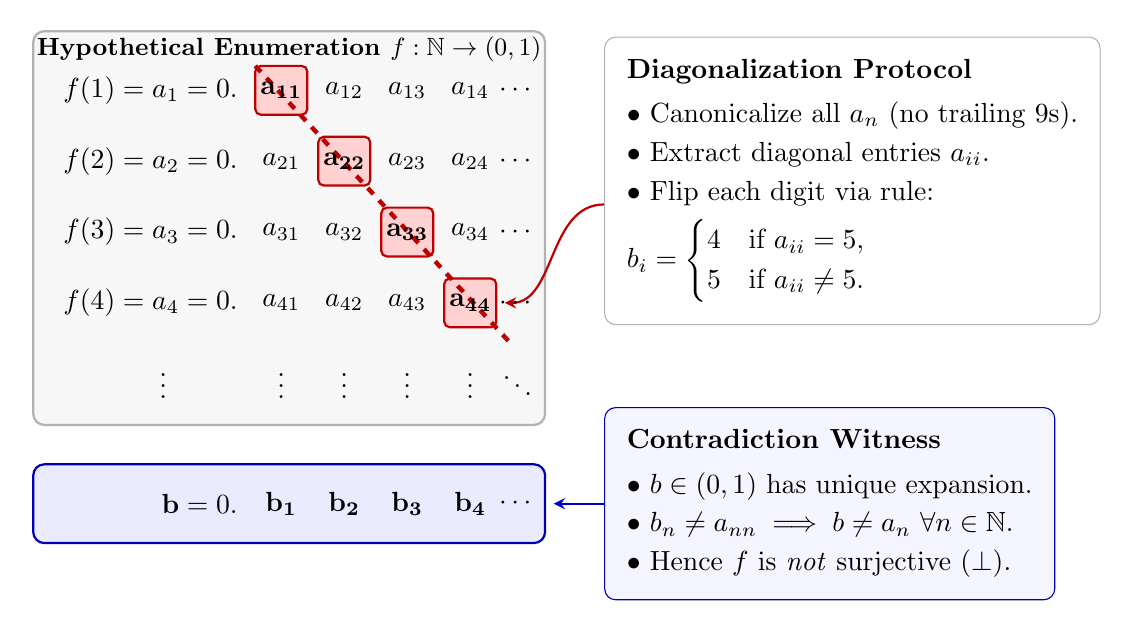
\begin{tikzpicture}[scale=1.0]
    % LAYER 1: Fills and shaded regions
    \fill[gray!6, rounded corners=4pt] (-0.3, -0.25) rectangle (6.2, 4.75);
    \fill[blue!8, rounded corners=4pt] (-0.3, -1.75) rectangle (6.2, -0.75);
    % Highlighted diagonal digit cells
    \fill[red!18, rounded corners=2pt] (2.52, 3.69) rectangle (3.18, 4.31);
    \fill[red!18, rounded corners=2pt] (3.32, 2.79) rectangle (3.98, 3.41);
    \fill[red!18, rounded corners=2pt] (4.12, 1.89) rectangle (4.78, 2.51);
    \fill[red!18, rounded corners=2pt] (4.92, 0.99) rectangle (5.58, 1.61);

    % LAYER 2: Borders, frames, and structural lines
    \draw[thick, gray!60, rounded corners=4pt] (-0.3, -0.25) rectangle (6.2, 4.75);
    \draw[thick, blue!70!black, rounded corners=4pt] (-0.3, -1.75) rectangle (6.2, -0.75);
    \draw[thick, red!75!black, rounded corners=2pt] (2.52, 3.69) rectangle (3.18, 4.31);
    \draw[thick, red!75!black, rounded corners=2pt] (3.32, 2.79) rectangle (3.98, 3.41);
    \draw[thick, red!75!black, rounded corners=2pt] (4.12, 1.89) rectangle (4.78, 2.51);
    \draw[thick, red!75!black, rounded corners=2pt] (4.92, 0.99) rectangle (5.58, 1.61);

    % LAYER 3: Diagonal guide and off-axis callout arrows
    \draw[ultra thick, red!75!black, dashed] (2.52, 4.31) -- (5.75, 0.80);
    \draw[->, >=stealth, thick, red!75!black, shorten >=2pt] (6.95, 2.55) to[out=180, in=0] (5.62, 1.30);
    \draw[->, >=stealth, thick, blue!80!black, shorten >=2pt] (6.95, -1.25) -- (6.24, -1.25);

    % LAYER 4: Text nodes and labels (explicit black color)
    % Header inside enumeration box
    \node[black, font=\small\bfseries] at (2.95, 4.52) {Hypothetical Enumeration $f : \mathbb{N} \to (0, 1)$};

    % Row 1
    \node[black, anchor=east] at (2.42, 4.0) {$f(1) = a_1 = 0.$};
    \node[black] at (2.85, 4.0) {$\mathbf{a_{11}}$};
    \node[black] at (3.65, 4.0) {$a_{12}$};
    \node[black] at (4.45, 4.0) {$a_{13}$};
    \node[black] at (5.25, 4.0) {$a_{14}$};
    \node[black] at (5.85, 4.0) {$\cdots$};

    % Row 2
    \node[black, anchor=east] at (2.42, 3.1) {$f(2) = a_2 = 0.$};
    \node[black] at (2.85, 3.1) {$a_{21}$};
    \node[black] at (3.65, 3.1) {$\mathbf{a_{22}}$};
    \node[black] at (4.45, 3.1) {$a_{23}$};
    \node[black] at (5.25, 3.1) {$a_{24}$};
    \node[black] at (5.85, 3.1) {$\cdots$};

    % Row 3
    \node[black, anchor=east] at (2.42, 2.2) {$f(3) = a_3 = 0.$};
    \node[black] at (2.85, 2.2) {$a_{31}$};
    \node[black] at (3.65, 2.2) {$a_{32}$};
    \node[black] at (4.45, 2.2) {$\mathbf{a_{33}}$};
    \node[black] at (5.25, 2.2) {$a_{34}$};
    \node[black] at (5.85, 2.2) {$\cdots$};

    % Row 4
    \node[black, anchor=east] at (2.42, 1.3) {$f(4) = a_4 = 0.$};
    \node[black] at (2.85, 1.3) {$a_{41}$};
    \node[black] at (3.65, 1.3) {$a_{42}$};
    \node[black] at (4.45, 1.3) {$a_{43}$};
    \node[black] at (5.25, 1.3) {$\mathbf{a_{44}}$};
    \node[black] at (5.85, 1.3) {$\cdots$};

    % Vertical ellipses
    \node[black] at (1.35, 0.35) {$\vdots$};
    \node[black] at (2.85, 0.35) {$\vdots$};
    \node[black] at (3.65, 0.35) {$\vdots$};
    \node[black] at (4.45, 0.35) {$\vdots$};
    \node[black] at (5.25, 0.35) {$\vdots$};
    \node[black] at (5.85, 0.35) {$\ddots$};

    % Constructed anti-diagonal element b
    \node[black, anchor=east] at (2.42, -1.25) {$\mathbf{b} = 0.$};
    \node[black] at (2.85, -1.25) {$\mathbf{b_1}$};
    \node[black] at (3.65, -1.25) {$\mathbf{b_2}$};
    \node[black] at (4.45, -1.25) {$\mathbf{b_3}$};
    \node[black] at (5.25, -1.25) {$\mathbf{b_4}$};
    \node[black] at (5.85, -1.25) {$\cdots$};

    % Anchored Legend / Annotation Node 1 (Top Right)
    \node[black, align=left, anchor=west, draw=gray!60, fill=white, rounded corners=4pt, inner sep=8pt] at (6.95, 2.85) {
        \textbf{Diagonalization Protocol}\\[4pt]
        $\bullet$ Canonicalize all $a_n$ (no trailing $9$s).\\[2pt]
        $\bullet$ Extract diagonal entries $a_{ii}$.\\[2pt]
        $\bullet$ Flip each digit via rule:\\[4pt]
        $\displaystyle b_i = \begin{cases} 4 & \text{if } a_{ii} = 5, \\ 5 & \text{if } a_{ii} \neq 5. \end{cases}$
    };

    % Anchored Legend / Annotation Node 2 (Bottom Right)
    \node[black, align=left, anchor=west, draw=blue!70!black, fill=blue!4, rounded corners=4pt, inner sep=8pt] at (6.95, -1.25) {
        \textbf{Contradiction Witness}\\[4pt]
        $\bullet$ $b \in (0, 1)$ has unique expansion.\\[2pt]
        $\bullet$ $b_n \neq a_{nn} \implies b \neq a_n\ \forall n \in \mathbb{N}$.\\[2pt]
        $\bullet$ Hence $f$ is \emph{not} surjective ($\bot$).
    };
\end{tikzpicture}
\caption{Visual architecture of Cantor's diagonalization argument proving that $(0, 1)$ is uncountable (Theorem 11.9).}
\label{fig:cantor_diag}
\end{figure}

\begin{figure}[htbp]
\centering
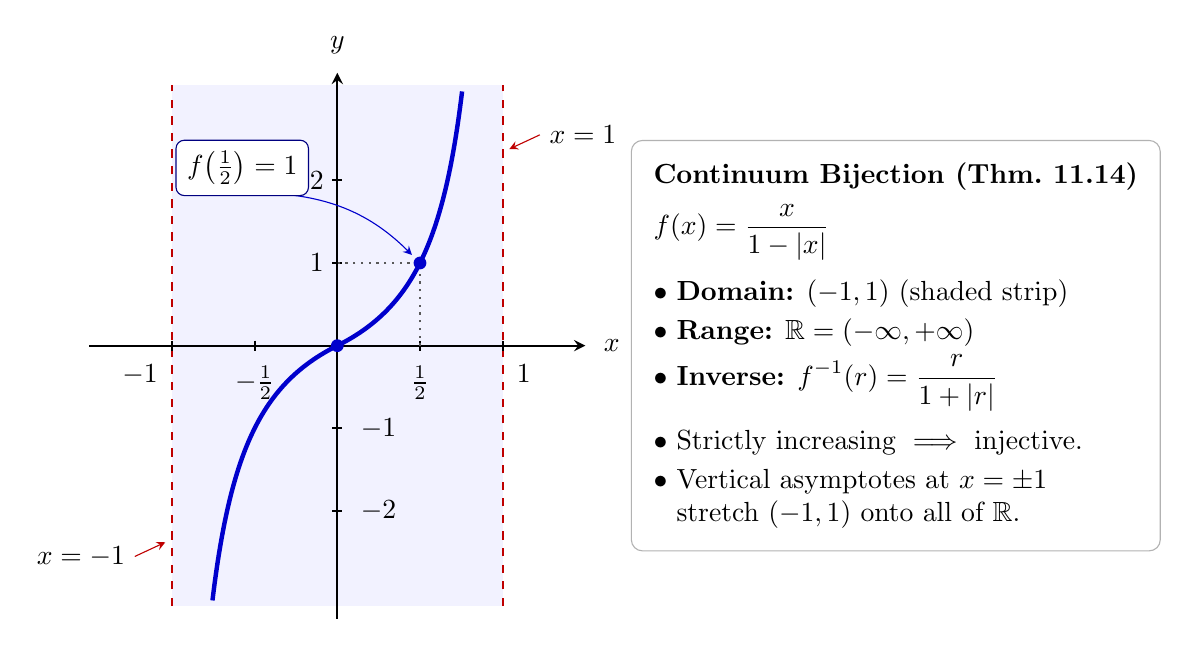
\begin{tikzpicture}[scale=1.05]
    % Note: Horizontal coordinate is scaled by u = 2x so (-1, 1) spans [-2, 2] cleanly.
    % LAYER 1: Shaded domain strip (-1, 1)
    \fill[blue!5] (-2, -3.15) rectangle (2, 3.15);

    % LAYER 2: Axes, vertical asymptotes, and microscopic tick marks
    \draw[->, >=stealth, thick, black] (-3.0, 0) -- (3.0, 0) node[right=3pt, black] {$x$};
    \draw[->, >=stealth, thick, black] (0, -3.3) -- (0, 3.3) node[above=3pt, black] {$y$};
    \draw[dashed, thick, red!75!black] (-2, -3.15) -- (-2, 3.15);
    \draw[dashed, thick, red!75!black] (2, -3.15) -- (2, 3.15);

    % Microscopic ticks on x-axis
    \draw[thick, black] (-2, 0.06) -- (-2, -0.06) node[below left=2pt, black] {$-1$};
    \draw[thick, black] (-1, 0.06) -- (-1, -0.06) node[below=2pt, black] {$-\frac{1}{2}$};
    \draw[thick, black] (1, 0.06) -- (1, -0.06) node[below=2pt, black] {$\frac{1}{2}$};
    \draw[thick, black] (2, 0.06) -- (2, -0.06) node[below right=2pt, black] {$1$};

    % Microscopic ticks on y-axis
    \draw[thick, black] (-0.06, 1) -- (0.06, 1) node[left=3pt, black] {$1$};
    \draw[thick, black] (-0.06, 2) -- (0.06, 2) node[left=3pt, black] {$2$};
    \draw[thick, black] (-0.06, -1) -- (0.06, -1) node[right=3pt, black] {$-1$};
    \draw[thick, black] (-0.06, -2) -- (0.06, -2) node[right=3pt, black] {$-2$};

    % Sample correspondence projection lines for x = 1/2 (u = 1) -> y = 1
    \draw[dotted, thick, gray!70!black] (1, 0) -- (1, 1) -- (0, 1);

    % LAYER 3: Primary bijection curve y = x/(1 - |x|) = u/(2 - |u|)
    \draw[ultra thick, blue!80!black, smooth, samples=80, domain=0:1.51] plot (\x, {\x/(2 - \x)});
    \draw[ultra thick, blue!80!black, smooth, samples=80, domain=-1.51:0] plot (\x, {\x/(2 + \x)});
    \fill[blue!80!black] (1, 1) circle (2.2pt);
    \fill[blue!80!black] (0, 0) circle (2.2pt);

    % Off-axis callout arrows
    \draw[->, >=stealth, thin, red!75!black, shorten >=2pt] (2.45, 2.55) -- (2.02, 2.35);
    \draw[->, >=stealth, thin, red!75!black, shorten >=2pt] (-2.45, -2.55) -- (-2.02, -2.35);
    \draw[->, >=stealth, thin, blue!80!black, shorten >=2pt] (-1.05, 1.85) to[out=0, in=135] (0.95, 1.05);

    % LAYER 4: Labels and anchored legend box
    \node[black, anchor=west] at (2.45, 2.55) {$x = 1$};
    \node[black, anchor=east] at (-2.45, -2.55) {$x = -1$};
    \node[black, align=center, fill=white, draw=blue!50!black, rounded corners=3pt, inner sep=4pt] at (-1.15, 2.15) {$\displaystyle f\!\left(\tfrac{1}{2}\right) = 1$};

    \node[black, align=left, anchor=west, draw=gray!60, fill=white, rounded corners=4pt, inner sep=8pt] at (3.55, 0.0) {
        \textbf{Continuum Bijection (Thm.~11.14)}\\[4pt]
        $\displaystyle f(x) = \frac{x}{1 - |x|}$\\[6pt]
        $\bullet$ \textbf{Domain:} $(-1, 1)$ (shaded strip)\\[2pt]
        $\bullet$ \textbf{Range:} $\mathbb{R} = (-\infty, +\infty)$\\[2pt]
        $\bullet$ \textbf{Inverse:} $\displaystyle f^{-1}(r) = \frac{r}{1 + |r|}$\\[6pt]
        $\bullet$ Strictly increasing $\implies$ injective.\\[2pt]
        $\bullet$ Vertical asymptotes at $x = \pm 1$\\
        \phantom{$\bullet$ }stretch $(-1, 1)$ onto all of $\mathbb{R}$.
    };
\end{tikzpicture}
\caption{Geometric representation of the bijection $f : (-1, 1) \to \mathbb{R}$ proving $|(-1, 1)| = |\mathbb{R}|$.}
\label{fig:bijection_plot}
\end{figure}

\subsection{Heuristics and ``Cheats''}

When confronted with an unseen cardinality problem, apply the following decision heuristic:
\begin{enumerate}
    \item \textbf{Need to prove a set $S$ is uncountable?} Never diagonalize if you can embed or take complements! First ask:
    \begin{itemize}
        \item Does $S$ contain an open interval $(a, b)$ or a copy of $\mathbb{R}$? If yes, apply Theorem 11.10 directly.
        \item Is $S = U \setminus C$ where $U$ is uncountable and $C$ is countable? If yes, prove by contradiction using countable union closure.
        \item Only if $S$ is an abstract space of infinite sequences or functions (e.g., $\{0, 1\}^{\mathbb{N}}$) should you deploy Cantor's diagonalization directly.
    \end{itemize}
    \item \textbf{Need to prove $|A| = |B|$ for two intervals or rays?}
    \begin{itemize}
        \item Bounded open to bounded open: use an affine map $\varphi(x) = mx + c$.
        \item Bounded open $(-M, M)$ to $\mathbb{R}$: use $\frac{x}{M - |x|}$ (easiest algebraic proof), $\frac{x}{M^2 - x^2}$ (smooth $C^\infty$ algebraic proof), or $\tan\left(\frac{\pi x}{2M}\right)$ (trigonometric proof).
        \item Unbounded line $\mathbb{R}$ to ray $(c, \infty)$: use $f(x) = e^x + c$.
        \item Chain existing bijections via composition whenever the question does not mandate a single explicit formula!
    \end{itemize}
    \item \textbf{Shortcut for verifying injectivity and surjectivity simultaneously:} If you construct an explicit candidate inverse $h : B \to A$ and verify both compositions $(h \circ f)(x) = x$ for all $x \in A$ and $(f \circ h)(y) = y$ for all $y \in B$ (along with verifying $f(A) \subseteq B$ and $h(B) \subseteq A$), you prove bijectivity in one clean algebraic stroke!
\end{enumerate}

\subsection{Pitfalls and Fallacies}

\begin{itemize}
    \item \textbf{The Dual Decimal Trap:} Choosing $b_i \neq a_{ii}$ without excluding $0$ and $9$ (e.g., setting $b_i = (a_{ii} + 1) \bmod 10$) fails to prevent $b$ from equaling an already listed terminating rational in disguise (such as $b = 0.4999\cdots = 0.5000\cdots$).
    \item \textbf{The False Downward Monotonicity Fallacy:} Assuming that if $A \subseteq B$ and $B$ is uncountable and $A$ is infinite, then $A$ must be uncountable. Counterexample: $\mathbb{N} \subset \mathbb{R}$ is infinite, $\mathbb{R}$ is uncountable, yet $\mathbb{N}$ is denumerable. Uncountability propagates \emph{upward} to supersets, never downward to subsets.
    \item \textbf{The Proper Subset Cardinality Trap:} Assuming $C \subsetneq D$ implies $|C| < |D|$. For infinite sets, proper containment is fully compatible with equinumerosity (e.g., $(0, 1) \subsetneq (0, 2) \subsetneq \mathbb{R}^+ \subsetneq \mathbb{R}$, yet all four sets have identical cardinality!).
    \item \textbf{Domain Neglect in Surjectivity Proofs:} Solving $f(x) = r$ algebraically for $x$ and substituting back into $f(x)$ without proving $x \in \operatorname{Dom}(f)$. As seen in Exercise 11.25, the quadratic $rx^2 + x - r = 0$ has a spurious root that satisfies the algebraic identity $\frac{x}{1-x^2} = r$ yet lies strictly \emph{outside} $(-1, 1)$!
    \item \textbf{Closure Failure Under Infinite Intersections:} Assuming that because every set $A_n$ in a nested sequence $A_1 \supseteq A_2 \supseteq \cdots$ is uncountable, the infinite intersection $\bigcap_{n=1}^{\infty} A_n$ must be uncountable. Counterexample: $\bigcap_{n=1}^{\infty} \left(-\frac{1}{n}, \frac{1}{n}\right) = \{0\}$ has cardinality $1$.
\end{itemize}

\section{Conceptual Synthesis and the Big Picture}

\subsection{Thematic Connections}

The unifying theme of Section 11.3 is \textbf{Bijective Invariance and the Discrete–Continuum Schism}. Earlier sections introduced equivalence relations and functions as structural tools; here, bijections serve as the universal measuring rod of set size. Two sets are indistinguishable in pure set theory if an invertible map translates between them.

Under this lens, infinity fractures into fundamentally incompatible realms. On one side lies the \emph{discrete infinite} ($\aleph_0 = |\mathbb{N}| = |\mathbb{Z}| = |\mathbb{Q}|$), characterized by sequential listability and algorithmic enumerability. On the other side lies the \emph{continuum} ($\mathfrak{c} = |(0, 1)| = |\mathbb{R}|$), which is structurally resistant to any countable listing. Remarkably, while metric geometry distinguishes $(0, 1)$ from $(-2, 2)$ and $\mathbb{R}$ via length and compactness, pure cardinality collapses all of them into a single equivalence class. Furthermore, Exercise 11.20 reveals a striking asymmetry inside the real line: although $\mathbb{Q}$ is topologically dense in $\mathbb{R}$, almost every real number is irrational—the rationals form a negligibly thin, countable skeleton embedded in an overwhelmingly uncountable sea of irrationals.

\subsection{Forward and Backward Links}

\textbf{Backward Links:} Section 11.3 builds directly on foundational function theory (injectivity, surjectivity, inverses, and compositions) and the first two sections of Chapter 11 (equivalence of numerical cardinality, denumerability of $\mathbb{Z}$ and $\mathbb{Q}$, and Theorem 11.4 on infinite subsets of denumerable sets). Without the prior proof that $\mathbb{Q}$ is denumerable, Exercise 11.20 could not deduce the uncountability of $\mathbb{I}$ from $\mathbb{R} = \mathbb{Q} \cup \mathbb{I}$.

\textbf{Forward Links:} The questions raised at the end of Section 11.3—specifically whether there exist \emph{three or more} distinct infinite cardinalities and how to formally define $|A| < |B|$—launch directly into advanced mathematics:
\begin{itemize}
    \item \textbf{Orderings of Cardinality and Cantor's Theorem:} Defining $|A| \le |B|$ via injections and proving $|A| < |\mathcal{P}(A)|$ for every set $A$ (using a generalized diagonalization argument), establishing an infinite tower of strictly larger infinities $|\mathbb{N}| < |\mathbb{R}| < |\mathcal{P}(\mathbb{R})| < \cdots$, alongside the Cantor–Schr\"oder–Bernstein Theorem and the Continuum Hypothesis (CH).
    \item \textbf{Measure Theory and Axiomatic Probability:} Because $\mathbb{R}$ is uncountable and probability measures are only \emph{countably} additive ($\sigma$-additive), one cannot compute the probability of a continuous interval $[a, b]$ by summing the probabilities of its individual points (each point has Lebesgue measure zero). This exact obstruction necessitates Borel $\sigma$-algebras, Lebesgue integration, and probability density functions.
    \item \textbf{Computability Theory and Theoretical Computer Science:} The set of all finite-length computer programs (Turing machines) is countable, whereas the set of all functions $f : \mathbb{N} \to \{0, 1\}$ is uncountable (having cardinality $|\mathbb{R}|$). By Theorem 11.13, almost all mathematical problems are uncomputable—and Alan Turing's proof of the undecidability of the Halting Problem is a direct incarnation of Cantor's diagonalization!
\end{itemize}

\section{Abstract Real-World Modeling (AI, ML, and Quantitative Finance)}

\subsection{Concrete Advanced Scenarios}

The distinction between countable and uncountable spaces—and the construction of smooth bijections between bounded intervals and $\mathbb{R}$—plays a decisive operational role in modern quantitative fields:

\begin{enumerate}
    \item \textbf{Stochastic Calculus and Continuous-Time Asset Pricing (Quantitative Finance):}
    In the Black–Scholes–Merton framework and stochastic volatility models (e.g., Heston, SABR), asset prices $\{S_t\}_{t \in [0, T]}$ evolve over an \emph{uncountable} time index set $[0, T]$ (numerically equivalent to $(0, 1)$ and $\mathbb{R}$). The underlying sample space of continuous price trajectories, $\Omega = C([0, T], \mathbb{R})$, is itself uncountable. Because every individual trajectory occurs with probability zero under the Wiener measure $\mathbb{P}$, events cannot be evaluated pointwise; instead, risk-neutral pricing requires defining expectations over Borel $\sigma$-algebras on uncountable spaces and ensuring pathwise regularity (e.g., via Kolmogorov's Continuity Theorem) so that uncountable suprema such as barrier-option payoffs $\sup_{t \in [0, T]} S_t$ remain measurable random variables.

    \item \textbf{Statistical Learning Theory and Generalization Bounds (Machine Learning):}
    When training a deep neural network or support vector machine, the parameter space $\Theta \subseteq \mathbb{R}^d$ generates an \emph{uncountable} hypothesis class $\mathcal{H} = \{h_\theta : \theta \in \Theta\}$. For a finite or countable hypothesis class, uniform convergence of empirical risk $\hat{R}_n(h)$ to true population risk $R(h)$ follows trivially from Hoeffding's inequality and a union bound. Because $\mathcal{H}$ is uncountable, a naive union bound sums uncountably many positive error probabilities and diverges vacuously. Overcoming this uncountability barrier motivated the entire apparatus of Vapnik–Chervonenkis (VC) dimension, Rademacher complexity, and $\varepsilon$-covering numbers—techniques that effectively project an uncountable function class onto a finite/countable skeleton at resolution $\varepsilon$.

    \item \textbf{Normalizing Flows and Constrained Diffeomorphic Reparameterization (Generative AI):}
    Modern generative models (Normalizing Flows, Variational Autoencoders, and Score-Based Diffusion Models) learn a smooth bijective map $T_\theta : \mathcal{Z} \to \mathcal{X}$ pushing forward a tractable base probability distribution $p_Z$ on $\mathbb{R}^d$ onto a complex data manifold $\mathcal{X}$. When modeling bounded physical or financial quantities—such as probabilities in $(0, 1)$, correlation matrices with entries in $(-1, 1)$, or positive volatilities in $\mathbb{R}^+$—exact continuum bijections (directly generalizing $f(x) = \frac{x}{1-|x|}$, $g(x) = \frac{x}{1-x^2}$, and $\exp : \mathbb{R} \to \mathbb{R}^+$) transform constrained inference into unconstrained Euclidean optimization while preserving exact likelihoods via the Jacobian change-of-variables formula.
\end{enumerate}

\subsection{Model Problem Setup: Diffeomorphic Stochastic Correlation Modeling in Quantitative Finance}

We construct a rigorous quantitative finance model that directly operationalizes the smooth continuum bijection $g : (-1, 1) \to \mathbb{R}$ from \textbf{Exercise 11.25} to guarantee boundary-respecting stochastic correlation dynamics in multi-asset derivative pricing.

\subsubsection{Probability Space and State Space Formulation}
Fix a finite trading horizon $T > 0$, noting that the continuous time index set $[0, T]$ is uncountable with $|[0, T]| = |(0, 1)| = |\mathbb{R}|$. Let $(\Omega, \mathcal{F}, \{\mathcal{F}_t\}_{t \in [0, T]}, \mathbb{P})$ be a complete filtered probability space satisfying the usual conditions, supporting a standard one-dimensional Brownian motion $\{W_t\}_{t \in [0, T]}$.

Suppose we wish to model the instantaneous stochastic correlation $\rho_t$ between two financial assets (e.g., an equity index and its stochastic volatility, or two sovereign yield factors). By the Cauchy–Schwarz inequality, any non-degenerate correlation must lie strictly within the bounded uncountable open interval
\[
\mathcal{S} = (-1, 1).
\]
Modeling $\rho_t$ directly via an unconstrained Gaussian Ornstein–Uhlenbeck process fails catastrophically because Gaussian distributions assign strictly positive probability mass to $\mathbb{R} \setminus (-1, 1)$, violating positive semi-definiteness of the covariance matrix.

\subsubsection{Bijective Transformation and Latent Dynamics}
Invoke the $C^\infty$-diffeomorphic bijection $g : (-1, 1) \to \mathbb{R}$ established in Exercise 11.25:
\[
X_t = g(\rho_t) = \frac{\rho_t}{1 - \rho_t^2} \in \mathbb{R},
\]
with its exact, globally well-defined algebraic inverse $\phi = g^{-1} : \mathbb{R} \to (-1, 1)$ proved in Exercise 11.25(a):
\[
\rho_t = \phi(X_t) = \begin{cases}
\displaystyle \frac{-1 + \sqrt{1 + 4X_t^2}}{2X_t} & \text{if } X_t \neq 0, \\[10pt]
0 & \text{if } X_t = 0.
\end{cases}
\]
Because $X_t$ takes values in the unconstrained space $\mathbb{R}$, we specify its latent dynamics as a mean-reverting Ornstein–Uhlenbeck Stochastic Differential Equation (SDE):
\begin{equation}
dX_t = \kappa\left(\bar{x} - X_t\right) dt + \sigma\, dW_t, \quad X_0 = g(\rho_0) \in \mathbb{R},
\end{equation}
where $\kappa > 0$ is the speed of mean reversion, $\bar{x} \in \mathbb{R}$ is the long-run latent mean, and $\sigma > 0$ is the volatility of latent correlation.

\subsubsection{Derivation of the Induced Bounded SDE via It\^o's Lemma}
To obtain the exact physical dynamics of $\rho_t = \phi(X_t)$ on $(-1, 1)$, we compute the first two derivatives of $\phi$ using the Inverse Function Theorem on $g(\rho) = \frac{\rho}{1 - \rho^2}$. Differentiating $g$ yields
\[
g'(\rho) = \frac{1 + \rho^2}{(1 - \rho^2)^2} > 0 \qquad \text{and} \qquad g''(\rho) = \frac{2\rho(3 + \rho^2)}{(1 - \rho^2)^3}.
\]
Consequently, for $\rho = \phi(x)$, the inverse derivatives are
\[
\phi'(x) = \frac{1}{g'(\rho)} = \frac{(1 - \rho^2)^2}{1 + \rho^2}, \qquad \phi''(x) = -\frac{g''(\rho)}{\left(g'(\rho)\right)^3} = -\frac{2\rho(3 + \rho^2)(1 - \rho^2)^3}{(1 + \rho^2)^3}.
\]
Since $\phi \in C^2(\mathbb{R})$, applying \textbf{It\^o's Lemma} to $\rho_t = \phi(X_t)$ gives
\[
d\rho_t = \left[\phi'(X_t)\,\kappa(\bar{x} - X_t) + \frac{1}{2}\sigma^2 \phi''(X_t)\right] dt + \sigma \phi'(X_t)\, dW_t.
\]
Substituting $X_t = g(\rho_t)$ and our closed-form expressions for $\phi'$ and $\phi''$ yields the autonomous, strictly boundary-preserving SDE for stochastic correlation on $(-1, 1)$:
\begin{equation}
d\rho_t = \left[\kappa\left(\bar{x} - \frac{\rho_t}{1 - \rho_t^2}\right)\frac{(1 - \rho_t^2)^2}{1 + \rho_t^2} - \sigma^2 \frac{\rho_t(3 + \rho_t^2)(1 - \rho_t^2)^3}{(1 + \rho_t^2)^3}\right] dt + \sigma \frac{(1 - \rho_t^2)^2}{1 + \rho_t^2}\, dW_t.
\end{equation}
Notice the remarkable boundary behavior inherited from the bijection $g$: as $\rho_t \to \pm 1$, the diffusion coefficient $\sigma \frac{(1 - \rho_t^2)^2}{1 + \rho_t^2} \to 0$ quadratically while the drift pulls $\rho_t$ strictly inward toward the interior of $(-1, 1)$, guaranteeing $\mathbb{P}\left(\rho_t \in (-1, 1)\ \forall t \in [0, T]\right) = 1$.

\subsubsection{Exact Transition Density and Maximum Likelihood Calibration Objective}
Because $X_t$ is Gaussian, conditioned on $\mathcal{F}_{t_{k-1}}$ at discrete observation times $0 = t_0 < t_1 < \cdots < t_N = T$ with step $\Delta t = t_k - t_{k-1}$, $X_{t_k} \mid X_{t_{k-1}} \sim \mathcal{N}(\mu_k, v^2)$, where
\[
\mu_k = X_{t_{k-1}} e^{-\kappa \Delta t} + \bar{x}\left(1 - e^{-\kappa \Delta t}\right), \qquad v^2 = \frac{\sigma^2}{2\kappa}\left(1 - e^{-2\kappa \Delta t}\right).
\]
By the measure-theoretic change-of-variables formula for the diffeomorphism $g : (-1, 1) \to \mathbb{R}$, the exact transition probability density of the observed correlation $\rho_{t_k}$ given $\rho_{t_{k-1}}$ is
\[
p_\theta\left(\rho_{t_k} \mid \rho_{t_{k-1}}\right) = \frac{1}{\sqrt{2\pi v^2}} \exp\left(-\frac{\left(g(\rho_{t_k}) - \mu_k\right)^2}{2v^2}\right) \cdot \left|g'(\rho_{t_k})\right|,
\]
where $\theta = (\kappa, \bar{x}, \sigma) \in \mathbb{R}^+ \times \mathbb{R} \times \mathbb{R}^+$ and $\left|g'(\rho)\right| = \frac{1 + \rho^2}{(1 - \rho^2)^2}$ is the exact Jacobian determinant. Calibrating the model from market correlation time series $\{\rho_{t_k}\}_{k=0}^N$ therefore reduces to minimizing the exact negative log-likelihood loss function:
\[
\mathcal{L}(\theta) = \sum_{k=1}^{N} \left[\frac{1}{2}\ln\left(2\pi v^2\right) + \frac{\left(g(\rho_{t_k}) - \mu_k(\theta)\right)^2}{2v^2} - \ln\left(1 + \rho_{t_k}^2\right) + 2\ln\left(1 - \rho_{t_k}^2\right)\right],
\]
subject to $\kappa > 0$ and $\sigma > 0$ (which can themselves be unconstrained via the Exercise 11.24 bijection $\kappa = e^{\eta_1},\ \sigma = e^{\eta_2}$ for $\eta_1, \eta_2 \in \mathbb{R}$).

\section{Common Variations and Untested Concepts}

While Section 11.3 focuses on open intervals, $\mathbb{R}$, $\mathbb{I}$, and $\mathbb{C}$, standard university courses routinely test four crucial extensions that do not appear in the assigned exercises. Below, we formalize and rigorously prove each variation.

\subsection{Variation 1: Closed and Half-Open Intervals Are Equinumerous With Open Intervals}

A major omission in Exercises 11.20--11.25 is handling endpoints: how does one map the \emph{closed} interval $[0, 1]$ bijectively onto the \emph{open} interval $(0, 1)$? No continuous bijection can exist (since $[0, 1]$ is compact and $(0, 1)$ is not), so one must use a piecewise ``Hilbert's Hotel'' shift on an embedded countably infinite sequence.

\begin{proposition}
The closed interval $[0, 1]$ and the open interval $(0, 1)$ are numerically equivalent: $|[0, 1]| = |(0, 1)|$.
\end{proposition}

\begin{proof}
Identify the denumerable subset $D = \left\{\frac{1}{n} : n \in \mathbb{N},\ n \ge 2\right\} = \left\{\frac{1}{2}, \frac{1}{3}, \frac{1}{4}, \dots\right\} \subset (0, 1)$. Define $f : [0, 1] \to (0, 1)$ by absorbing the two boundary points $0$ and $1$ into the front of the sequence $D$ and shifting every element of $D$ forward by two slots:
\[
f(x) = \begin{cases}
\displaystyle \frac{1}{2} & \text{if } x = 0, \\[8pt]
\displaystyle \frac{1}{3} & \text{if } x = 1, \\[8pt]
\displaystyle \frac{1}{n + 2} & \text{if } x = \frac{1}{n} \text{ for some } n \in \mathbb{N},\ n \ge 2, \\[8pt]
x & \text{if } x \in (0, 1) \setminus D.
\end{cases}
\]
\emph{Well-Definedness:} Every branch outputs an element strictly inside $(0, 1)$, and the four input domains $\{0\}$, $\{1\}$, $D$, and $(0, 1) \setminus D$ form a pairwise disjoint partition of $[0, 1]$.

\emph{Injectivity:} The image of $\{0, 1\} \cup D$ is $\left\{\frac{1}{2}, \frac{1}{3}\right\} \cup \left\{\frac{1}{4}, \frac{1}{5}, \dots\right\} = D$, while the image of $(0, 1) \setminus D$ is $(0, 1) \setminus D$. Since these two image sets are disjoint, and $f$ is manifestly injective on each piece (in particular, $\frac{1}{n_1 + 2} = \frac{1}{n_2 + 2} \implies n_1 = n_2$), $f$ is injective on $[0, 1]$.

\emph{Surjectivity:} Let $y \in (0, 1)$. If $y = \frac{1}{2}$, then $y = f(0)$. If $y = \frac{1}{3}$, then $y = f(1)$. If $y = \frac{1}{k}$ for some integer $k \ge 4$, then $k - 2 \ge 2$ and $y = f\left(\frac{1}{k - 2}\right)$. Finally, if $y \in (0, 1) \setminus D$, then $y = f(y)$. Thus $f$ is surjective.

Therefore, $f : [0, 1] \to (0, 1)$ is bijective, so $|[0, 1]| = |(0, 1)|$.
\end{proof}

\subsection{Variation 2: Uncountability of Infinite Binary Sequence Space $\{0, 1\}^{\mathbb{N}}$}

In probability theory (infinite coin tosses) and theoretical computer science (bitstreams), one frequently works with the space $S = \{0, 1\}^{\mathbb{N}}$ of all infinite binary sequences $(x_1, x_2, x_3, \dots)$ with $x_k \in \{0, 1\}$. Diagonalization here is even cleaner than on $(0, 1)$ because there is no dual-representation ambiguity.

\begin{proposition}
The set $S = \{0, 1\}^{\mathbb{N}}$ of all infinite binary sequences is uncountable.
\end{proposition}

\begin{proof}
Assume, to the contrary, that $S$ is countable. Since $S$ is infinite (it contains the distinct sequences $e^{(k)}$ having a single $1$ in position $k$ and $0$s elsewhere), $S$ is denumerable. Thus there exists a bijection $f : \mathbb{N} \to S$. Denote $f(n) = s^{(n)} = \left(s^{(n)}_1, s^{(n)}_2, s^{(n)}_3, \dots\right)$ where $s^{(n)}_j \in \{0, 1\}$ for all $n, j \in \mathbb{N}$.

Construct a new binary sequence $t = (t_1, t_2, t_3, \dots) \in S$ by flipping every diagonal bit:
\[
t_k = 1 - s^{(k)}_k \quad \text{for every } k \in \mathbb{N}.
\]
Since $s^{(k)}_k \in \{0, 1\}$, we have $t_k \in \{0, 1\}$, so $t \in S$. For any $n \in \mathbb{N}$, the $n$-th coordinates of $t$ and $s^{(n)}$ satisfy $t_n = 1 - s^{(n)}_n \neq s^{(n)}_n$. Because two sequences are equal if and only if they agree in every coordinate, $t \neq s^{(n)} = f(n)$ for all $n \in \mathbb{N}$. Hence $f$ is not surjective, contradicting bijectivity. Therefore, $S$ is uncountable.
\end{proof}

\subsection{Variation 3: General Removal of Countable Subsets From Uncountable Sets}

Exercise 11.20 proved that $\mathbb{R} \setminus \mathbb{Q}$ is uncountable. This is a special case of a universal stability theorem for uncountable sets.

\begin{proposition}
Let $A$ be an uncountable set and let $C$ be any countable set. Then $A \setminus C$ is uncountable.
\end{proposition}

\begin{proof}
Assume, to the contrary, that $A \setminus C$ is countable. Let $B = A \cap C$. Since $B \subseteq C$ and $C$ is countable, $B$ is countable (by Theorem 11.4 if $B$ is infinite, or trivially if $B$ is finite). Observe that
\[
A = (A \setminus C) \cup (A \cap C) = (A \setminus C) \cup B, \qquad (A \setminus C) \cap B = \emptyset.
\]
If both $A \setminus C$ and $B$ are finite, then $A$ is finite, hence countable. If at least one of $A \setminus C$ or $B$ is denumerable while the other is countable, then by the disjoint countable union Lemma proved in Exercise 11.20, their union $A$ is denumerable, hence countable. In either case, $A$ is countable, contradicting the hypothesis that $A$ is uncountable. Therefore, $A \setminus C$ is uncountable.
\end{proof}

\subsection{Variation 4: The Plane and Complex Numbers Have the Exact Same Cardinality as $\mathbb{R}$}

Exercise 11.21 only proved that $\mathbb{C}$ is uncountable. Remarkably, $\mathbb{C}$ is \emph{not} strictly larger than $\mathbb{R}$: $|\mathbb{C}| = |\mathbb{R}^2| = |\mathbb{R}|$. Naive digit interleaving fails because of dual decimal expansions, so we exhibit a rigorous \textbf{non-terminating block-interleaving bijection}.

\begin{proposition}
The half-open unit square $(0, 1] \times (0, 1]$ and the half-open unit interval $(0, 1]$ are numerically equivalent. Consequently, $|\mathbb{R}^2| = |\mathbb{C}| = |\mathbb{R}|$.
\end{proposition}

\begin{proof}
Every number $x \in (0, 1]$ possesses a \emph{strictly unique non-terminating} decimal expansion $x = 0.d_1 d_2 d_3 \cdots$ containing infinitely many nonzero digits (for instance, $1 = 0.9999\cdots$ and $0.5 = 0.4999\cdots$). Because infinitely many digits are nonzero, every such expansion decomposes uniquely into an infinite sequence of finite digit blocks $(B_1, B_2, B_3, \dots)$, where each block $B_k$ consists of zero or more $0$s followed by a single nonzero digit $d \in \{1, 2, \dots, 9\}$ (for example, $0.005704\cdots$ decomposes into $B_1 = 005$, $B_2 = 7$, $B_3 = 04$, $\dots$). Conversely, concatenating any infinite sequence of such blocks yields a unique non-terminating decimal expansion in $(0, 1]$.

Define $\Phi : (0, 1] \times (0, 1] \to (0, 1]$ as follows: given $(x, y) \in (0, 1] \times (0, 1]$ with unique block decompositions $x = 0.X_1 X_2 X_3 \cdots$ and $y = 0.Y_1 Y_2 Y_3 \cdots$, set
\[
\Phi(x, y) = 0.X_1 Y_1 X_2 Y_2 X_3 Y_3 \cdots.
\]
\emph{Well-Definedness:} Because each block $X_k$ and $Y_k$ ends in a nonzero digit, the interleaved expansion has infinitely many nonzero digits and therefore represents a valid non-terminating decimal in $(0, 1]$.

\emph{Injectivity:} Suppose $\Phi(x, y) = \Phi(x', y')$. Since non-terminating decimal expansions are unique and every block terminates immediately upon encountering a nonzero digit, scanning the common expansion left-to-right uniquely recovers every block: $X_k = X'_k$ and $Y_k = Y'_k$ for all $k \in \mathbb{N}$. Hence $x = x'$ and $y = y'$.

\emph{Surjectivity:} Let $z \in (0, 1]$ have unique non-terminating block decomposition $z = 0.Z_1 Z_2 Z_3 Z_4 \cdots$. Define $x = 0.Z_1 Z_3 Z_5 \cdots \in (0, 1]$ and $y = 0.Z_2 Z_4 Z_6 \cdots \in (0, 1]$. Both expansions contain infinitely many nonzero digits and satisfy $\Phi(x, y) = z$.

Thus $\Phi$ is bijective, proving $|(0, 1] \times (0, 1]| = |(0, 1]|$. Since $|(0, 1]| = |(0, 1)| = |\mathbb{R}|$ (by the Hilbert's Hotel shift of Variation 1 absorbing the single endpoint $1$, combined with Corollary 11.15), it follows immediately that $|\mathbb{C}| = |\mathbb{R} \times \mathbb{R}| = |(0, 1] \times (0, 1]| = |(0, 1]| = |\mathbb{R}|$.
\end{proof}

\section{Advanced Diagnostic Testing: ``Find the Flaw''}

Each of the five proofs below appears polished and persuasive at first reading, yet conceals a \emph{single, critical mathematical or logical flaw}. Act as a rigorous referee: locate the exact invalid step, explain why it breaks the argument, and formulate the correct resolution. Verify your diagnosis against the Solution Key in Section~\ref{sec:solution_key}.

\subsection{Diagnostic Problem 1: A Simplified Diagonalization Proof of Theorem 11.9}

\textbf{Claim:} The open interval $(0, 1)$ is uncountable.

\textbf{Proposed Proof:} Assume, to the contrary, that $(0, 1)$ is denumerable, so there exists a bijection $f : \mathbb{N} \to (0, 1)$. Write each $a_n = f(n)$ in its canonical decimal expansion $a_n = 0.a_{n1}a_{n2}a_{n3}\cdots$ that does not repeat $9$ from any point onward. Define a real number $b = 0.b_1 b_2 b_3 \cdots$ by setting
\[
b_i = \begin{cases}
9 & \text{if } a_{ii} = 0, \\
0 & \text{if } a_{ii} \neq 0,
\end{cases}
\]
for every $i \in \mathbb{N}$. Clearly $b \in (0, 1)$, and for every $n \in \mathbb{N}$, the $n$-th digit of $b$ satisfies $b_n \neq a_{nn}$. Therefore, $b \neq a_n$ for all $n \in \mathbb{N}$, contradicting the surjectivity of $f$. Hence $(0, 1)$ is uncountable. $\blacksquare$

\subsection{Diagnostic Problem 2: Proving the Rationals in $(0, 1)$ Are Uncountable}

\textbf{Claim:} The set $S = \mathbb{Q} \cap (0, 1)$ of rational numbers in $(0, 1)$ is uncountable.

\textbf{Proposed Proof:} Assume, to the contrary, that $S$ is countable. Since $S$ is infinite, $S$ is denumerable, so there exists a bijection $f : \mathbb{N} \to S$. For each $n \in \mathbb{N}$, write $f(n) = q_n = 0.q_{n1}q_{n2}q_{n3}\cdots$ using the terminating decimal expansion whenever $q_n$ has two expansions. Construct $b = 0.b_1 b_2 b_3 \cdots$ by setting $b_i = 4$ if $q_{ii} = 5$ and $b_i = 5$ if $q_{ii} \neq 5$. Because $b$ contains only the digits $4$ and $5$, $b$ has a unique decimal expansion and satisfies $0.4 < b < 0.6$, so $b \in (0, 1)$. Moreover, $b_n \neq q_{nn}$ for every $n \in \mathbb{N}$, so $b \neq q_n$ for every $n \in \mathbb{N}$. Thus $f$ is not onto, a contradiction. Therefore, $S$ is uncountable. $\blacksquare$

\subsection{Diagnostic Problem 3: Uncountability of a Nested Infinite Intersection}

\textbf{Claim:} The infinite intersection $I = \bigcap_{n=1}^{\infty} \left(-\frac{1}{n}, \frac{1}{n}\right)$ is uncountable.

\textbf{Proposed Proof:} We first prove by mathematical induction that for every $k \in \mathbb{N}$, the finite intersection $I_k = \bigcap_{n=1}^{k} \left(-\frac{1}{n}, \frac{1}{n}\right)$ is uncountable.
\begin{itemize}
    \item \emph{Base Case ($k = 1$):} $I_1 = (-1, 1)$, which is numerically equivalent to $\mathbb{R}$ by Theorem 11.14 and hence uncountable.
    \item \emph{Inductive Step:} Assume $I_k = \left(-\frac{1}{k}, \frac{1}{k}\right)$ is uncountable. Then
    \[
    I_{k+1} = I_k \cap \left(-\frac{1}{k+1}, \frac{1}{k+1}\right) = \left(-\frac{1}{k+1}, \frac{1}{k+1}\right).
    \]
    By Exercise 11.23(c), $\left(-\frac{1}{k+1}, \frac{1}{k+1}\right)$ has the same cardinality as $(0, 1)$, which is uncountable by Theorem 11.9.
\end{itemize}
By the Principle of Mathematical Induction, $I_k$ is uncountable for every $k \in \mathbb{N}$. Passing to the limit as $k \to \infty$, we conclude that $I = \bigcap_{n=1}^{\infty} \left(-\frac{1}{n}, \frac{1}{n}\right)$ is uncountable. $\blacksquare$

\subsection{Diagnostic Problem 4: Alternative Surjectivity Proof for $g(x) = \frac{x}{1 - x^2}$}

\textbf{Claim:} The function $g : (-1, 1) \to \mathbb{R}$ defined by $g(x) = \frac{x}{1 - x^2}$ is surjective.

\textbf{Proposed Proof:} Let $r \in \mathbb{R}$. If $r = 0$, then $x = 0 \in (-1, 1)$ satisfies $g(0) = 0$. Now suppose $r \neq 0$, and define
\[
x = \frac{-1 - \sqrt{1 + 4r^2}}{2r}.
\]
Because $1 + 4r^2 > 1$, the radical is real and $x$ is well-defined. Expanding $x^2$ gives
\[
x^2 = \frac{1 + 2\sqrt{1 + 4r^2} + (1 + 4r^2)}{4r^2} = \frac{1 + 2r^2 + \sqrt{1 + 4r^2}}{2r^2},
\]
and therefore
\[
1 - x^2 = \frac{2r^2 - \left(1 + 2r^2 + \sqrt{1 + 4r^2}\right)}{2r^2} = \frac{-1 - \sqrt{1 + 4r^2}}{2r^2}.
\]
Notice that $-1 - \sqrt{1 + 4r^2} < -2 \neq 0$. Dividing $x$ by $1 - x^2$ yields
\[
g(x) = \frac{x}{1 - x^2} = \frac{\frac{-1 - \sqrt{1 + 4r^2}}{2r}}{\frac{-1 - \sqrt{1 + 4r^2}}{2r^2}} = r.
\]
Hence every $r \in \mathbb{R}$ has a preimage under $g$, proving $g$ is surjective. $\blacksquare$

\subsection{Diagnostic Problem 5: Naive Digit Interleaving Bijection $(0, 1) \times (0, 1) \to (0, 1)$}

\textbf{Claim:} Defining $F : (0, 1) \times (0, 1) \to (0, 1)$ by mapping the unique canonical (no trailing $9$s) decimal expansions $x = 0.x_1 x_2 x_3 \cdots$ and $y = 0.y_1 y_2 y_3 \cdots$ to
\[
F(x, y) = 0.x_1 y_1 x_2 y_2 x_3 y_3 \cdots
\]
yields a surjective function onto $(0, 1)$.

\textbf{Proposed Proof:} Let $z \in (0, 1)$ be arbitrary, written in its unique canonical decimal expansion $z = 0.z_1 z_2 z_3 z_4 \cdots$ with no trailing $9$s. Split the digits of $z$ into odd-indexed and even-indexed subsequences by defining
\[
x = 0.z_1 z_3 z_5 \cdots \qquad \text{and} \qquad y = 0.z_2 z_4 z_6 \cdots.
\]
Since $z$ has no trailing $9$s, neither $x$ nor $y$ can have trailing $9$s, and both lie in $(0, 1)$. Interleaving their digits immediately gives $F(x, y) = 0.z_1 z_2 z_3 z_4 \cdots = z$. Therefore, $F$ is surjective. $\blacksquare$

\subsection{Solution Key to Diagnostic Problems}
\label{sec:solution_key}

\begin{enumerate}
    \item \textbf{Flaw in Problem 1 (Violating the No-Trailing-$0$ / No-Trailing-$9$ Guard):}
    The proof commits \emph{two} fatal errors stemming from choosing digits $\{0, 9\}$:
    \begin{itemize}
        \item First, $b$ is not even guaranteed to lie in $(0, 1)$! If $a_{ii} \neq 0$ for all $i \in \mathbb{N}$, then $b = 0.000\cdots = 0 \notin (0, 1)$; conversely, if $a_{ii} = 0$ for all $i \in \mathbb{N}$, then $b = 0.999\cdots = 1 \notin (0, 1)$.
        \item Second, even if $b \in (0, 1)$, $b$ could end in an infinite string of $9$s—for instance, $b = 0.0999\cdots = 0.1000\cdots$—which equals an already listed number $a_k = 0.1000\cdots$ despite differing from $a_k$ in the $k$-th digit!
    \end{itemize}
    \textbf{Correction:} Restrict the constructed digits of $b$ to any two digits in $\{1, 2, \dots, 8\}$ (such as $\{4, 5\}$), ensuring $b \in (0, 1)$ and guaranteeing $b$ has a strictly unique decimal representation.

    \item \textbf{Flaw in Problem 2 (Failure to Verify Codomain Membership $b \in S$):}
    Every algebraic step is valid \emph{except} the hidden assumption that $b \in S = \mathbb{Q} \cap (0, 1)$! To contradict the surjectivity of $f : \mathbb{N} \to S$, the missing witness $b$ \emph{must belong to the codomain $S$}. While $b \in (0, 1)$, there is zero guarantee that $b$ is \emph{rational} (its decimal expansion of $4$s and $5$s need not be eventually periodic—and indeed, since $\mathbb{Q} \cap (0, 1)$ \emph{is} countable, $b$ is forced to be irrational!).
    \textbf{Resolution:} The claim itself is false because $\mathbb{Q} \cap (0, 1) \subseteq \mathbb{Q}$ is an infinite subset of a denumerable set, hence denumerable by Theorem 11.4.

    \item \textbf{Flaw in Problem 3 (Illegitimate Passage From Finite Induction to Infinite Intersection):}
    Mathematical induction proves a property $P(k)$ for every \emph{finite} integer $k \in \mathbb{N}$; it does \emph{not} prove $P(\infty)$. Although every finite intersection $I_k = (-1/k, 1/k)$ is uncountable, the infinite intersection is
    \[
    I = \bigcap_{n=1}^{\infty} \left(-\frac{1}{n}, \frac{1}{n}\right) = \{0\},
    \]
    because for any $x \neq 0$, the Archimedean Property provides $N \in \mathbb{N}$ with $1/N < |x|$, so $x \notin (-1/N, 1/N)$. Thus $|I| = 1$, which is finite and countable!
    \textbf{Resolution:} Never pass cardinality properties through an infinite intersection by induction; uncountability is not preserved under countable intersections.

    \item \textbf{Flaw in Problem 4 (Spurious Root Outside the Domain $(-1, 1)$):}
    Although the algebraic manipulation $g(x) = r$ is formally correct on $\mathbb{R} \setminus \{-1, 1\}$, the proof \emph{never checks whether $x \in (-1, 1)$}. In fact, for \emph{every} $r \neq 0$,
    \[
    |x| = \frac{1 + \sqrt{1 + 4r^2}}{2|r|} > \frac{1 + \sqrt{4r^2}}{2|r|} = \frac{1 + 2|r|}{2|r|} = 1 + \frac{1}{2|r|} > 1,
    \]
    so $x \notin (-1, 1)$! The chosen root always lies outside the domain of $g$, rendering $g(x)$ undefined for the given function $g : (-1, 1) \to \mathbb{R}$.
    \textbf{Correction:} Select the opposite quadratic root $x = \frac{-1 + \sqrt{1 + 4r^2}}{2r}$ and explicitly prove $|x| < 1$ via $\sqrt{1 + 4r^2} < 1 + 2|r|$, as executed in Exercise 11.25(a).

    \item \textbf{Flaw in Problem 5 (Subsequences Can Acquire Trailing $9$s or Collapse to $0$):}
    The assertion ``Since $z$ has no trailing $9$s, neither $x$ nor $y$ can have trailing $9$s, and both lie in $(0, 1)$'' is \textbf{false}! Consider the completely valid canonical real number
    \[
    z = 0.19090909\cdots = \frac{19}{99} - \frac{1}{11} + \cdots \in (0, 1),
    \]
    which alternates $0$s and $9$s after the first digit and therefore has \emph{no} trailing $9$s. Splitting its digits yields
    \[
    x = 0.1000\cdots = \frac{1}{10} \in (0, 1) \qquad \text{and} \qquad y = 0.9999\cdots = 1 \notin (0, 1)!
    \]
    Even worse, for $z = 0.29191919\cdots \in (0, 1)$, $x = 0.2111\cdots \in (0, 1)$ and $y = 0.9999\cdots = 1 \notin (0, 1)$, while for $z = 0.19290909\cdots$, $y = 0.9999\cdots$ violates the canonical no-trailing-$9$s condition. Thus $F$ is \emph{not} surjective onto $(0, 1)$.
    \textbf{Correction:} Replace single-digit interleaving with the non-terminating \emph{block-interleaving} bijection on $(0, 1] \times (0, 1]$ constructed in Section 7.4 (Variation 4), or apply the Cantor–Schr\"oder–Bernstein Theorem.
\end{enumerate}

\end{document}